\documentclass[a4paper,12pt]{extreport}
\usepackage[T2A]{fontenc}
\usepackage[utf8]{inputenc}
\usepackage{graphicx}
\usepackage[usenames]{color}
\usepackage{cite}
\usepackage[english,russian]{babel}
\usepackage{amssymb,amsmath,latexsym,enumerate}
\usepackage{array,longtable,lscape}
\usepackage{indentfirst}
\usepackage{titlesec}
\usepackage{graphicx}
\usepackage{subfigure,epsfig}
\usepackage{caption2}
\usepackage[onehalfspacing]{setspace}
\usepackage{textcomp}
%\usepackage[strict]{changepage}
\renewcommand{\baselinestretch}{1.5}
\numberwithin{equation}{chapter}
\sloppy
\makeatletter
\renewcommand{\@biblabel}[1]{#1.}
\makeatother
\usepackage{geometry}
\geometry{left=3cm}
\geometry{right=1.5cm}
\geometry{top=2cm}
\geometry{bottom=2cm}
\titleformat{\chapter}[block]{\Large\bfseries}{\Large\thechapter.}{0.5em}{}[\vspace*{-1cm}]
\titleformat{\section}{\large\bfseries}{{\thesection}}{0.5em}{}
\titleformat{\subsection}[runin]{\normalfont\bfseries}{\thesubsection}{0.5ex}{}

%---END OF HEAD----------------------------------------------------------------------------

\begin{document}
\renewcommand{\contentsname}{\Large Содержание}
\renewcommand{\bibname}{\normalfont\Large\bfseries Список литературы}
\renewcommand{\figurename}{\normalfont Рис.\!}

\begin{titlepage}
	\begin{center}
		Министерство науки и высшего образования Российской Федерации \\
		НАЦИОНАЛЬНЫЙ ИССЛЕДОВАТЕЛЬСКИЙ ЯДЕРНЫЙ УНИВЕРСИТЕТ <<МИФИ>> \\*
		\hrulefill
	\end{center}
	
	\begin{center}
		ИНСТИТУТ ИНТЕЛЛЕКТУАЛЬНЫХ КИБЕРНЕТИЧЕСКИХ СИСТЕМ\\
		КАФЕДРА \textnumero 31 ПРИКЛАДНАЯ МАТЕМАТИКА
	\end{center}
	\vspace{1cm}
	
	\begin{flushright}
		На правах рукописи\\
		УДК \underline{\textcolor{red}{вписать УДК}}
	\end{flushright}
	
	\vspace{0.5em}
	
	\begin{center}
		ЕСИС АЛЕКСАНДР ИВАНОВИЧ
	\end{center}
	
	\vspace{1em}
	
	\begin{center}
		\large ГЕНЕРАТИВНАЯ ОПТИМИЗАЦИЯ ТОПОЛОГИИ КАНАЛЬНОГО РАДИАТОРА
	\end{center}
	
	\vspace{2em}
	
	\begin{center}
		\large{Выпускная квалификационная работа бакалавра}
	\end{center}
	
	\vspace{1em}
	
	\begin{center}
		Направление подготовки 01.03.02 <<Прикладная математика и информатика>>
	\end{center}
	
	\vspace{2.5em}
	
	%\begin{adjustwidth}{9.5cm}{}
	\hfill \begin{minipage}[t]{75mm}
		Выпускная квалификационная\\
		работа защищена\\
		<<\rule[0mm]{0.8cm}{0.1mm}>> \hrulefill \ 20\rule[0mm]{0.4cm}{0.1mm} г.\\
		Оценка \hrulefill\\
		Секретарь ГЭК \hrulefill \ Чмыхов М.А.
	\end{minipage}
	%\end{adjustwidth}
	
	\vspace{\fill}
	
	\begin{center}
		г. Москва 2024
	\end{center}
\end{titlepage}

\newpage
\thispagestyle{empty}
\vspace*{3cm}
\begin{center}
	\Large \textbf{ПОЯСНИТЕЛЬНАЯ ЗАПИСКА} \\
	\large {к выпускной квалификационной работе на тему:}
\end{center}

\vspace{1em}

\begin{center}
	\large ГЕНЕРАТИВНАЯ ОПТИМИЗАЦИЯ ТОПОЛОГИИ КАНАЛЬНОГО РАДИАТОРА
\end{center}

\vspace{5em}

\begin{flushleft}
	\begin{longtable}{lcl}
		Студент--дипломник           & \underline{\hspace{2.9cm}} & Есис А.И.                                    \\
		                             &                            &                                              \\
		Руководитель проекта         & \underline{\hspace{2.9cm}} & к.ф.-м.н., доцент Чмыхов М.А.                \\
		                             &                            &                                              \\
		Констультант                 & \underline{\hspace{2.9cm}} & д.ф.-м.н., профессор Василевский--Коган В.В. \\
		                             &                            &                                              \\
		Рецензент                    & \underline{\hspace{2.9cm}} & к.ф.-м.н., доцент Пельмень П.П.              \\
		                             &                            &                                              \\
		Зав.~кафедрой \textnumero 31 & \underline{\hspace{2.9cm}} & д.ф.-м.н., профессор Кудряшов Н.А.
	\end{longtable}
\end{flushleft}

%%-----------------------------------------------------------------------------

\tableofcontents
\setcounter{page}{3}

\chapter*{Введение}
\addcontentsline{toc}{chapter}{Введение}

Актуальность задачи эффективного охлаждения вычислительных систем и электронных устройств становится все более значимой в связи с постоянным ростом их мощности и миниатюризацией.
Увеличение производительности вычислительных систем, развитие электромобилей \cite{li_analysis_2022} и стремление к энергосбережению требуют разработки компактных и высокоэффективных систем охлаждения.
Неэффективное решение проблемы теплоотвода может привести к перегреву, снижению производительности и даже повреждению техники. 
Целью данного исследования является разработка и оптимизация геометрии радиатора для водяной системы охлаждения процессора с использованием методов вычислительной гидродинамики (CFD).
Для достижения поставленной цели были использованы программные пакеты SALOME \cite{wOfDocSalome}, OpenFOAM и решатель chtMultiRegionFoam \cite{wChtMultiRegionFoam}. 
Первым этапом работы было создание базовой геометрии и расчетной сетки в графическом интерфейсе SALOME.
Затем по полученной сетке проводилось численное моделирование с использованием OpenFOAM для оценки параметров каждой конструкции.
В качестве целевой функции оптимизации была выбрана функция, учитывающая общую теплопередачу и перепад давления \cite{mekki_genetic_2021}.
Входными параметрами оптимизации являлись значения заполнения доменов, причем каждая новая геометрия генерировалась автоматически с использованием скрипта на Python.
Для решения задачи оптимизации были применены и сравнены два алгоритма: эволюционный (генетический) и градиентный (BFGS) \cite{limited_BFGS}.
Результаты показали, что генетический алгоритм эффективнее справляется с глобальной оптимизацией в многомерных пространствах параметров, используя на 30-40\% меньше итераций \cite{Chernyshev2007}. 
Проведенное исследование подтвердило, что оптимизация геометрии и параметров системы охлаждения позволяет повысить ее эффективность на 7-10\% по сравнению с традиционными конструкциями, имеющими линейное и шахматное расположение элементов.
Полученные результаты могут быть использованы для разработки и улучшения радиаторов в различных инженерных областях, где необходим эффективный теплоотвод.

\chapter{Постановка задачи}
\section{Математическая модель процесса теплообмена}

\subsection{Уравнение энергии:}

\begin{equation}
	\rho c_p \frac{\partial T}{\partial t} + \nabla \cdot (\rho \mathbf{u} T) = \nabla \cdot (k \nabla T) + Q
\end{equation}

\subsection*{Уравнение движения:}

\begin{equation}
	\frac{\partial \rho}{\partial t} + \nabla \cdot (\rho \mathbf{u}) = 0
\end{equation}

\subsection{Уравнение состояния:}

\begin{equation}
	p = \rho R T
\end{equation}

\subsection*{Уравнение теплового баланса для источника тепла $Q$:}

\begin{equation}
	Q = V \cdot q
\end{equation}

\subsection{Граничные условия:}

\begin{itemize}
	\item \textbf{Вход воздуховода:}
	      \begin{align*}
		       & T|_\text{вход} = T_\text{вх} = 50 \, \text{К},     \\
		       & \mathbf{u}|_\text{вход} = (3, 0, 0) \, \text{м/с}.
	      \end{align*}
	\item \textbf{Выход воздуховода:}
	      \begin{align*}
		       & \frac{\partial T}{\partial n}\bigg|_\text{выход} = 0, \\
		       & p|_\text{выход} = 0 \, \text{Па}.
	      \end{align*}
	\item \textbf{Стенки воздуховода:} Условие прилипания и непроницаемости для скорости, теплоизолированные стенки.
	      \begin{align*}
		       & \mathbf{u}|_\text{стенки} = 0,                         \\
		       & \frac{\partial T}{\partial n}\bigg|_\text{стенки} = 0.
	      \end{align*}
	\item \textbf{На границах между подобластями:} Непрерывность температуры, потоков тепла и скорости.
\end{itemize}

\begin{enumerate}
	\item Воздуховод:
	      \[
		      \begin{aligned}
			       & -150 \leq x \leq 150 \\
			       & -20 \leq y \leq 30   \\
			       & 10 \leq z \leq 32    \\
		      \end{aligned}
	      \]
	      
	\item Нагреватель:
	      \[
		      \begin{aligned}
			       & -7.5 \leq x \leq 17.5 \\
			       & -7.5 \leq y \leq 17.5 \\
			       & 7.5 \leq z \leq 10    \\
		      \end{aligned}
	      \]
	      
	\item Подложка радиатора:
	      \[
		      \begin{aligned}
			       & -10 \leq x \leq 20 \\
			       & -10 \leq y \leq 20 \\
			       & 10 \leq z \leq 15  \\
		      \end{aligned}
	      \]
	      
	\item Цилиндр 1:
	      \[
		      \begin{aligned}
			       & -7.5 \leq x \leq -2.5 \\
			       & -7.5 \leq y \leq -2.5 \\
			       & 15 \leq z \leq 30     \\
		      \end{aligned}
	      \]
	      
	\item Цилиндр 2:
	      \[
		      \begin{aligned}
			       & 2.5 \leq x \leq 7.5 \\
			       & 2.5 \leq y \leq 7.5 \\
			       & 15 \leq z \leq 30   \\
		      \end{aligned}
	      \]
	      
	\item Цилиндр 3:
	      \[
		      \begin{aligned}
			       & 12.5 \leq x \leq 17.5 \\
			       & 12.5 \leq y \leq 17.5 \\
			       & 15 \leq z \leq 30     \\
		      \end{aligned}
	      \]
\end{enumerate}

\subsection{Начальные условия:}

\begin{itemize}
	\item \textbf{Температура:}
	      \begin{itemize}
		      \item $T_0 = 50 \, \text{С} \quad \text{(константная по всей области)}$
	      \end{itemize}
	      
	\item \textbf{Давление:}
	      \begin{itemize}
		      \item $p_0 = 0 \, \text{Па} \quad \text{(константное по всему воздуховоду)}$
	      \end{itemize}
	      
	\item \textbf{Теплоемкость материала (Cp):}
	      \begin{itemize}
		      \item Для меди: $C_p = 385 \, \text{Дж/(кг$\cdot$К)}$
		      \item Для воздуха: $C_p = 1005 \, \text{Дж/(кг$\cdot$К)}$
	      \end{itemize}
	      
	\item \textbf{Плотность материала ($\rho$):}
	      \begin{itemize}
		      \item Для меди: $\rho = 8900 \, \text{кг/м}^3$
		      \item Для воздуха: $\rho = 1.196 \, \text{кг/м}^3$
	      \end{itemize}
	      
	\item \textbf{Теплопроводность материала ($\kappa$):}
	      \begin{itemize}
		      \item Для меди: $\kappa = 400 \, \text{Вт/(м$\cdot$К)}$
	      \end{itemize}
	      
	\item \textbf{Вязкость материала ($\mu$):}
	      \begin{itemize}
		      \item Для воздуха: $\mu = 1.8 \times 10^{-5} \, \text{Па$\cdot$с}$
	      \end{itemize}
	      
	\item \textbf{Число Прандтля (Pr):}
	      \begin{itemize}
		      \item Для воздуха: $\text{Pr} = 0.7$
	      \end{itemize}
	      
	\item \textbf{Тепловой поток в источнике (q):}
	      \begin{itemize}
		      \item $q = 1.0 \times 10^7 \, \text{Вт/м}^3$
	      \end{itemize}
\end{itemize}

\section{Постановка задачи оптимизации}

Минимизировать максимальную температуру внутри нагревателя, перемещая цилиндры вдоль оси $x$:

\begin{equation*}
	\min_{x_1, x_2} \max_{(x, y) \in \Omega} T_h(x, y)
\end{equation*}

при условиях:

1. Уравнение теплопроводности для пластины:

\begin{equation*}
	\frac{\partial^2 T_{fin}}{\partial x^2} + \frac{\partial^2 T_{fin}}{\partial y^2} = 0, \quad (x, y) \in \Omega_{fin}
\end{equation*}

2. Граничные условия для пластины:

\begin{align*}
	T_{fin}(x, 0)                             & = T_{\text{duct}}, \quad x \in [0, L]                               \\
	\frac{\partial T_{fin}}{\partial y}(x, H) & = 0, \quad x \in [0, L]                                             \\
	\frac{\partial T_{fin}}{\partial x}(0, y) & = \frac{\partial T_{fin}}{\partial x}(L, y) = 0, \quad y \in [0, H]
\end{align*}

3. Уравнение теплопроводности для цилиндров:

\begin{align*}
	\frac{d^2 T_{c1}}{dx_1^2} & = 0, \quad x_1 \in [x_1 - R, x_1 + R] \\
	\frac{d^2 T_{c2}}{dx_2^2} & = 0, \quad x_2 \in [x_2 - R, x_2 + R]
\end{align*}

4. Граничные условия для цилиндров:

\begin{align*}
	T_{c1}(x_1 - R) & = T_{c1}(x_1 + R) = T_h \\
	T_{c2}(x_2 - R) & = T_{c2}(x_2 + R) = T_h
\end{align*}

5. Условия сопряжения на границе между пластиной и цилиндрами:

\begin{align*}
	T_{fin}(x, y_1)                             & = T_{c1}(x), \quad (x, y_1) \in \Gamma_{c1}             \\
	T_{fin}(x, y_2)                             & = T_{c2}(x), \quad (x, y_2) \in \Gamma_{c2}             \\
	\frac{\partial T_{fin}}{\partial y}(x, y_1) & = \frac{dT_{c1}}{dx}(x), \quad (x, y_1) \in \Gamma_{c1} \\
	\frac{\partial T_{fin}}{\partial y}(x, y_2) & = \frac{dT_{c2}}{dx}(x), \quad (x, y_2) \in \Gamma_{c2}
\end{align*}

6. Ограничения на положение цилиндров:

\begin{align*}
	-10 & \leq x_1 \leq 20 \\
	-10 & \leq x_2 \leq 20
\end{align*}

Здесь $\Omega_{fin}$ - область пластины, $\Gamma_{c1}$ и $\Gamma_{c2}$ - границы контакта между пластиной и цилиндрами, $L$ и $H$ - длина и высота пластины, $R$ - радиус цилиндров, $y_1$ и $y_2$ - координаты $y$ центров цилиндров.

\section{Первый этапа исследования}

На первом этапе исследования решалась задача охлаждения нагретого тела с помощью установки радиатора.

Геометрия радиатора строилась с использованием графического интерфейса SALOME. Этот этап позволил получить исходную геометрию, которая будет использоваться для последующих анализов.
Затем, для повышения гибкости и автоматизации процесса, был создан скрипт на языке Python, который генерирует геометрию радиатора. 
В этом скрипте можно устанавливать параметры радиатора, такие как расположение элементов.
Это позволяет быстро создавать и изменять различные варианты геометрии радиатора для дальнейшего анализа и оптимизации.

Для исследования применялись три различных варианта геометрии радиатора.
Примеры геометрии:
\begin{figure}[h]
	\begin{center}
		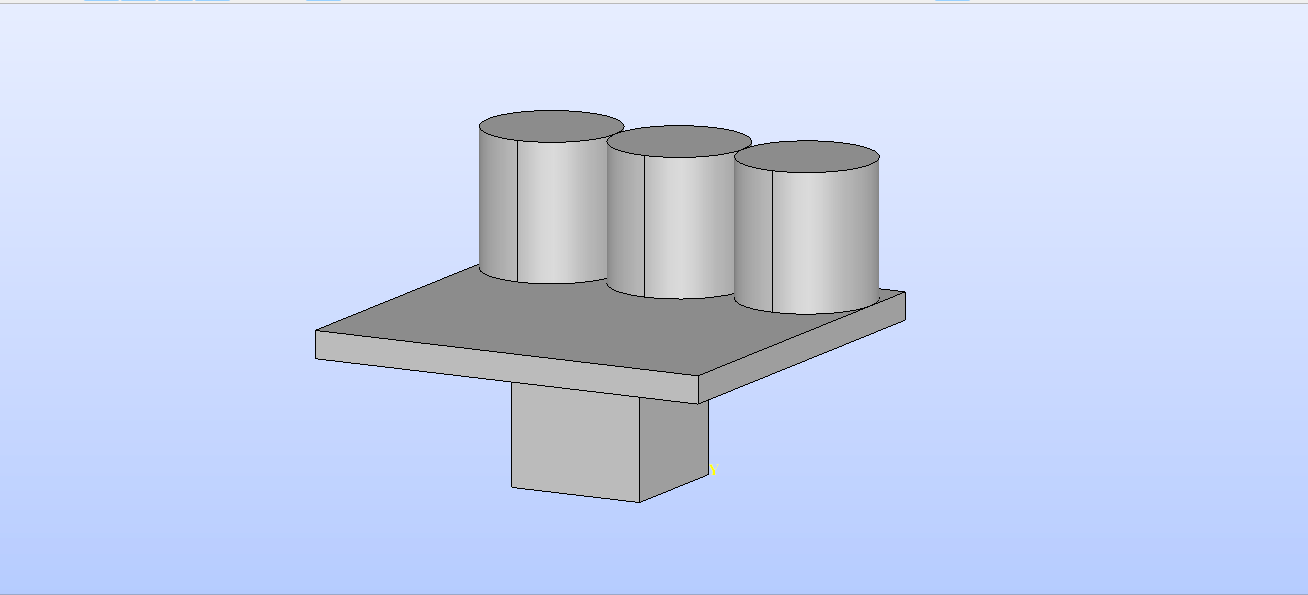
\includegraphics[width=0.5\linewidth]{images/1.1.png}
		\caption{Модель геометрии 1} %% подпись к рисунку
	\end{center}
\end{figure}
\begin{figure}[h]
	\begin{center}
		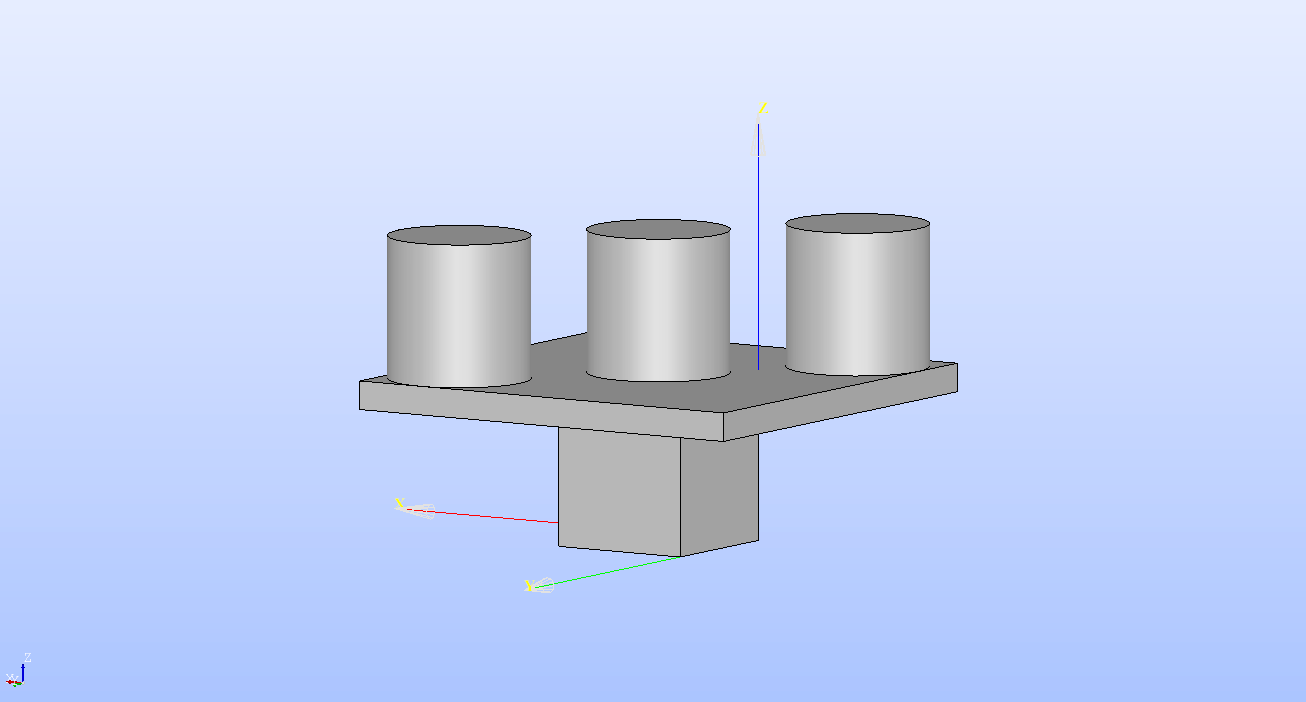
\includegraphics[width=0.5\linewidth]{images/1.2.png}
		\caption{Модель геометрии 2}
	\end{center}
\end{figure}
\begin{figure}[h]
	\begin{center}
		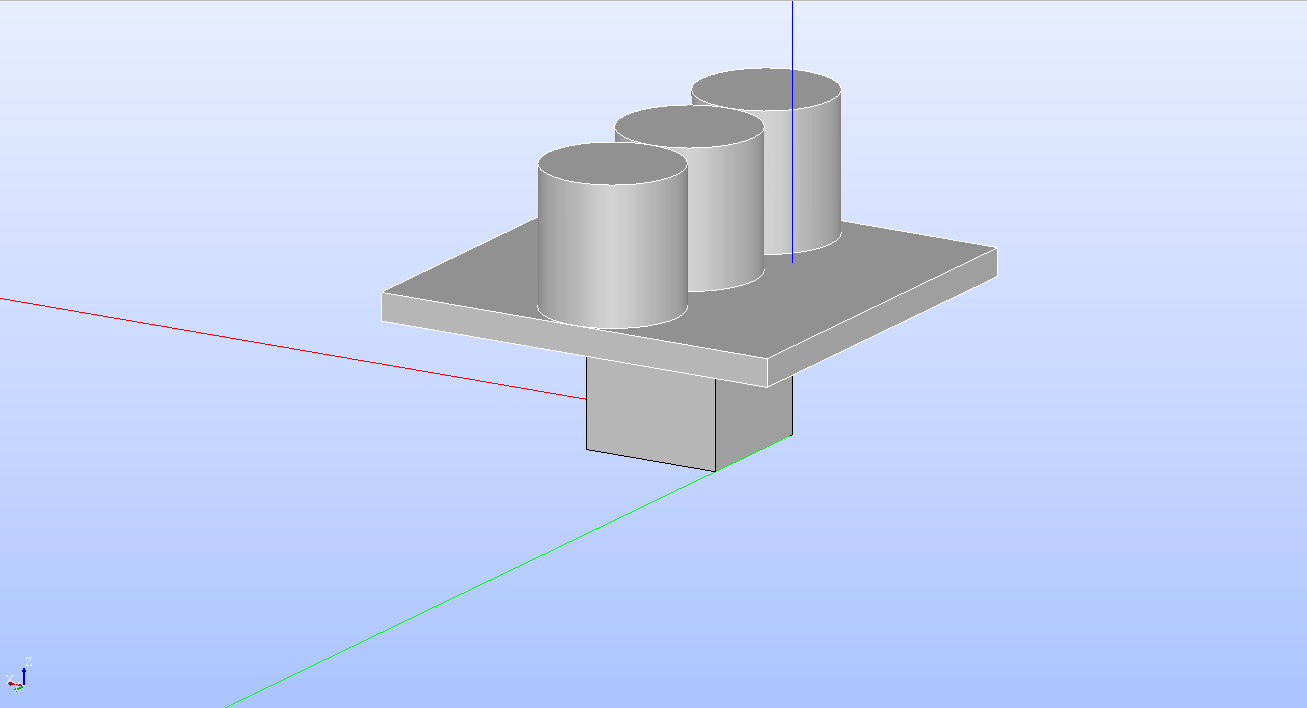
\includegraphics[width=0.5\linewidth]{images/1.3.png}
		\caption{Модель геометрии 3}
	\end{center}
\end{figure}
\newpage

\begin{figure}[h]
	\begin{center}
		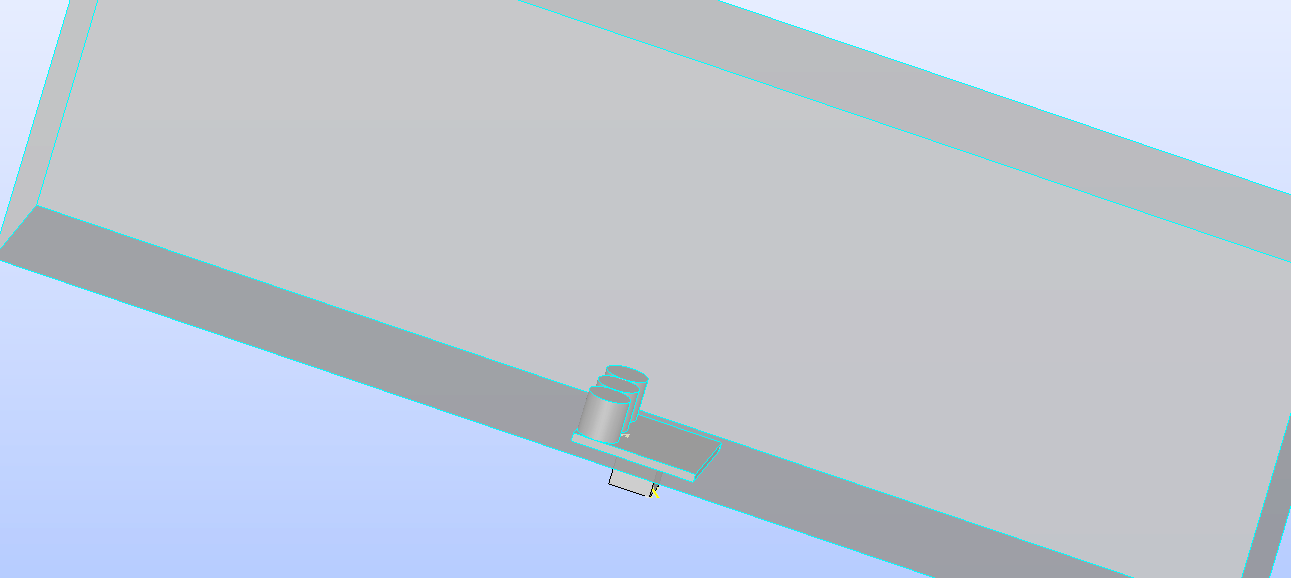
\includegraphics[width=0.5\linewidth]{images/2.1.png}
		\caption{Модель геометрии 1} %% подпись к рисунку
	\end{center}
\end{figure}
\begin{figure}[h]
	\begin{center}
		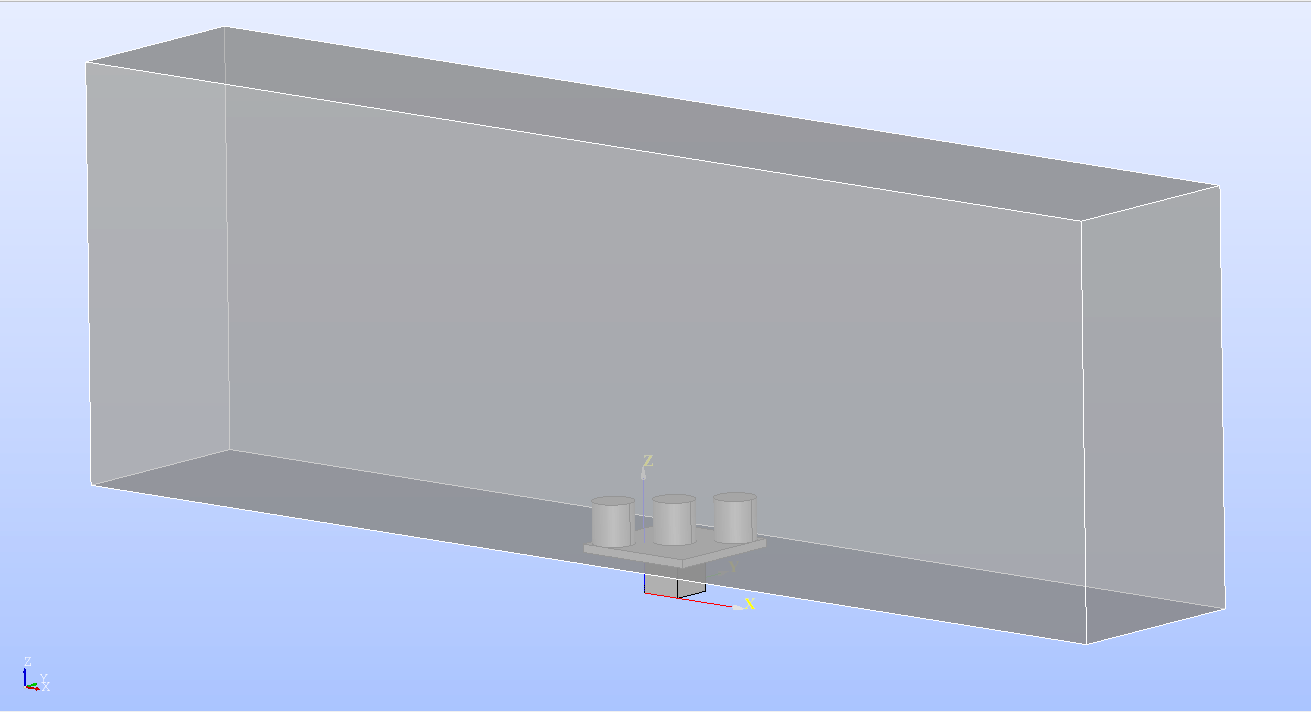
\includegraphics[width=0.5\linewidth]{images/2.2.png}
		\caption{Модель геометрии 2}
	\end{center}
\end{figure}
\newpage
\begin{figure}[h]
	\begin{center}
		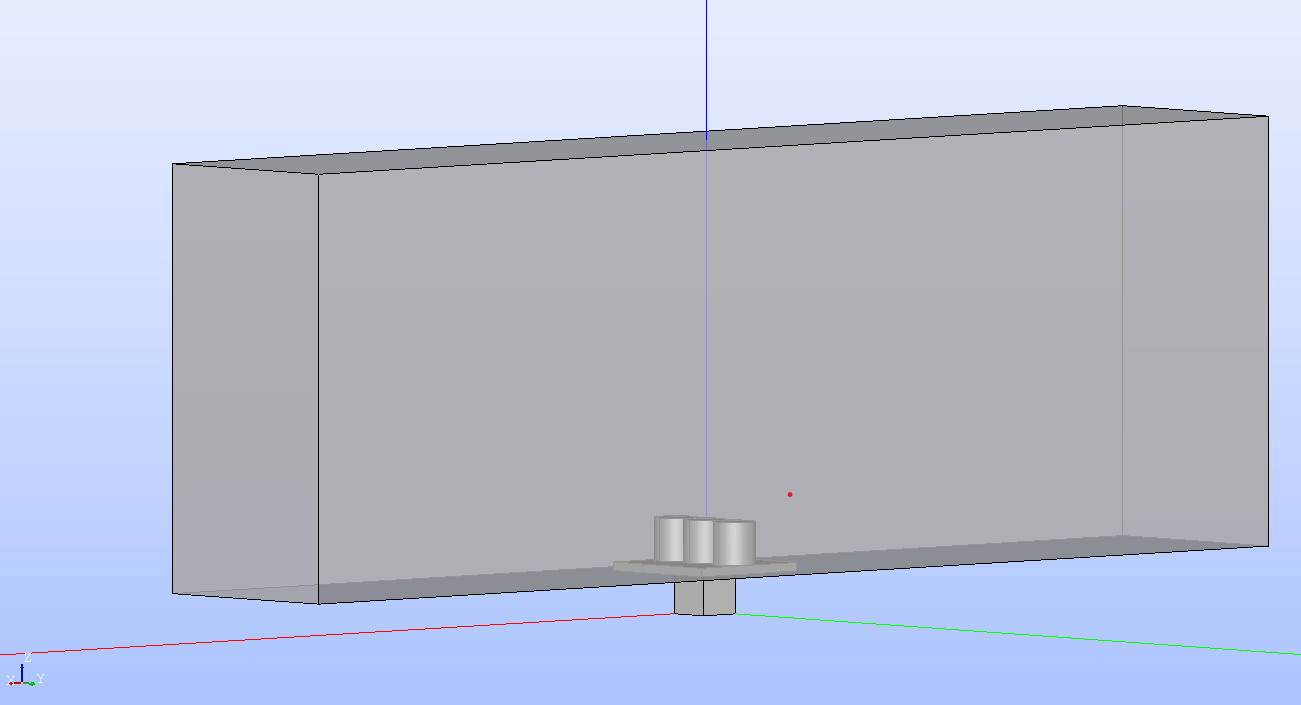
\includegraphics[width=0.5\linewidth]{images/2.3.png}
		\caption{Модель геометрии 3}
	\end{center}
\end{figure}

\par
В данных моделях части радиатора (3 цилиндрических элемента) являются подвижными и могут быть сдвинуты по оси Ox. Их радиус основания равен 5 мм, а высота 10 мм. 
Размеры подложки радиатора по ширине и длине 30 мм, а по высоте 2 мм. Нагреватель представляет собой куб с длиной ребра 10 мм и объемной плотностью источников тепла 2.94 * $10^7$ Вт/$м^3$. 
Скорость потока воздуха 5.6 м/с. Воздух находится в параллелепипеде размерами 300 мм по длине, 50 мм по ширине и 100 мм по высоте. Начальная температура –296.9 К. Параметры материалов приведены в таблице 1 \cite{aHeatTranserf}.

\begin{table}[h]
	\begin{tabular}{|l|l|l|l|}
		\hline
		                                          & Нагреватель & Радиатор & Воздух        \\
		Плотность {[}кг/$м^3${]}                  & 1280        & 2700     & 1.196         \\
		\hline
		Cp   {[}Дж/кг*К{]}                        & 1004        & 900      & 1005          \\
		\hline
		Коэффициент теплопроводности {[}Вт/м*К{]} & 80          & 200      &               \\
		\hline
		Молекулярная масса {[}г/моль{]}           & 50          & 27       & 28.9          \\
		\hline
		Вязкость {[}кг/м*с{]}                     &             &          & $1.8*10^{-5}$ \\
		\hline
		Число Прандтля                            &             &          & 0.7           \\
		\hline
	\end{tabular}
	\caption{Параметры задачи} %% подпись к рисунку
\end{table}

Затем по модели была построена сетка c уплотнением в области радиатора и нагревателя и произведено разбиение на регионы:

\begin{figure}[h]
	\begin{center}
		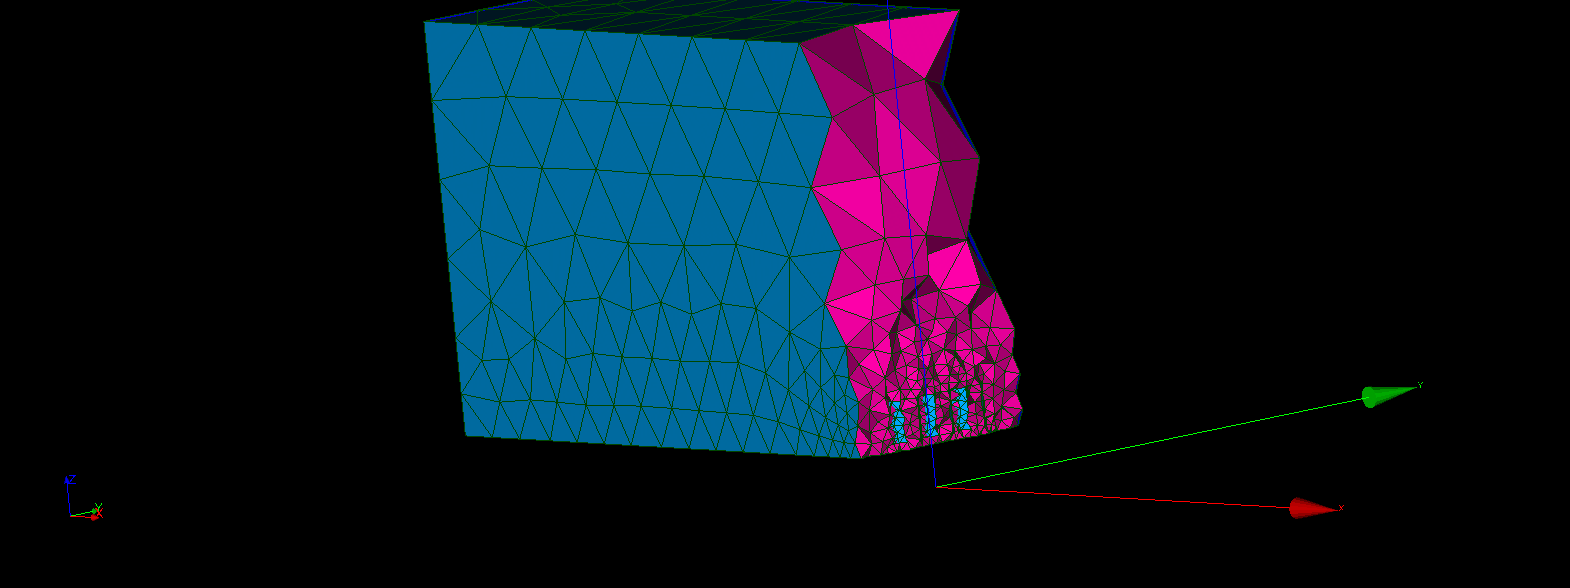
\includegraphics[width=0.35\linewidth]{images/3.png}
		\caption{Сетка модели 1} %% подпись к рисунку
	\end{center}
\end{figure}

\par
Для численного решения задачи используется решатель chtMultiRegionFoam.
Он применяется для расчета теплообмена между жидкостью/газом и твердым телом. А также для моделирования сложных задач, связанных с теплопередачей и теплообменом в многорегиональных системах \cite{wChtMultiRegionFoam}.
Для каждого региона задавались начальные и граничные условия. Были также заданы дополнительные функции для анализа \cite{aHeatTranserf}.
Для моделей были получены следующие результаты распределений по температурам:

\begin{figure}[h]
	\begin{center}
		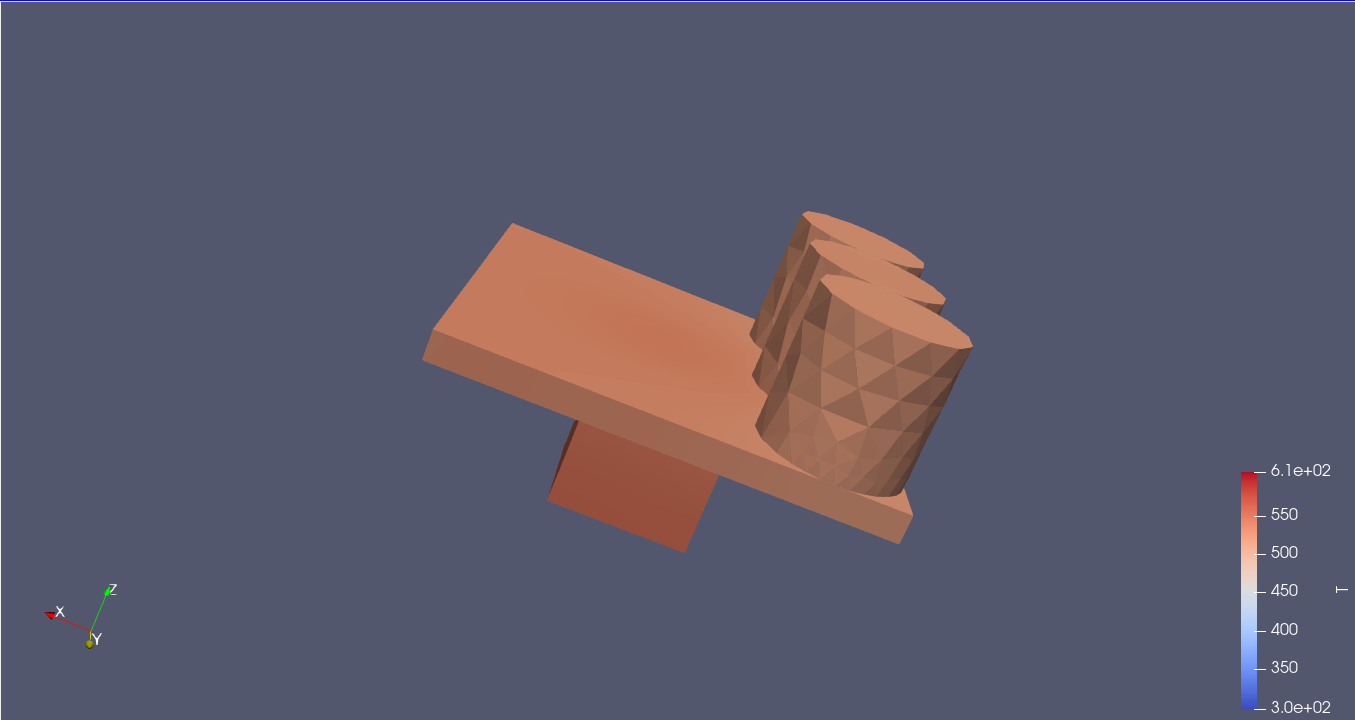
\includegraphics[width=0.45\linewidth]{images/5.1.png}
		\caption{Распределение температуры для модели 1} %% подпись к рисунку
	\end{center}
\end{figure}

\begin{figure}[h]
	\begin{center}
		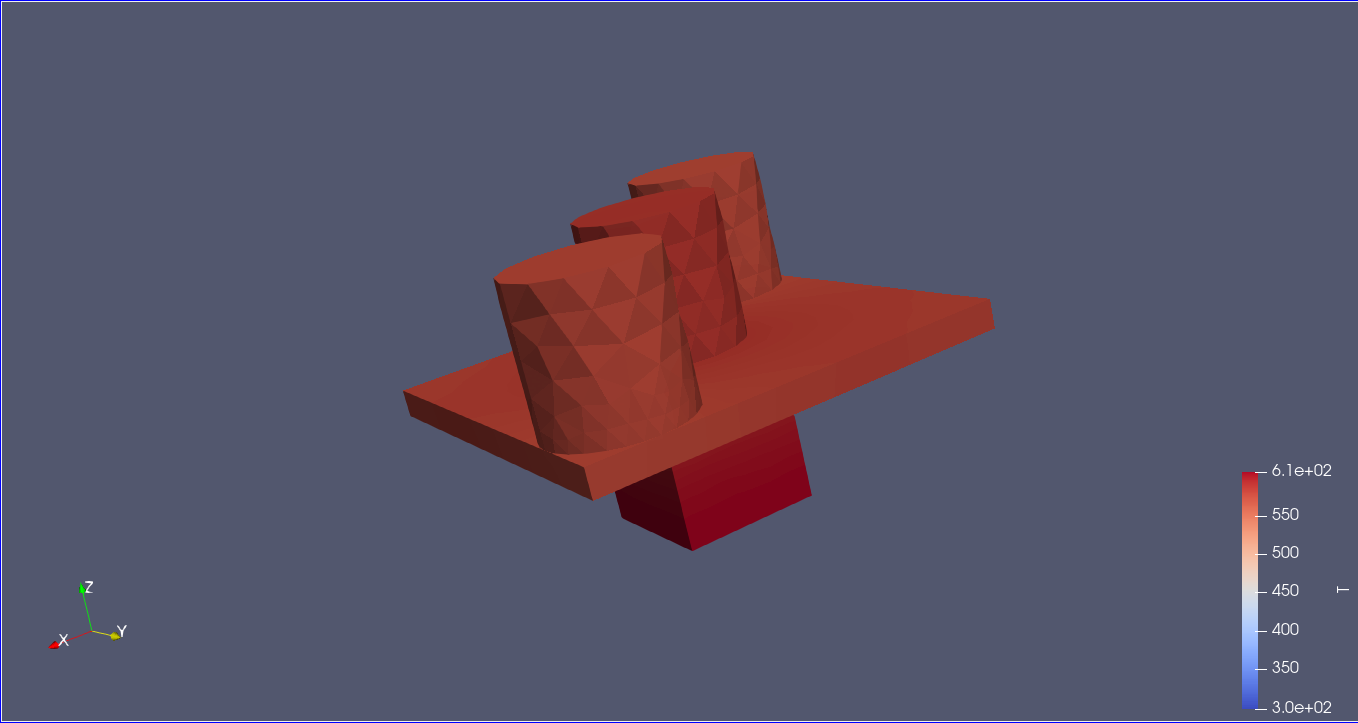
\includegraphics[width=0.45\linewidth]{images/5.2.png}
		\caption{Распределение температуры для модели 2} %% подпись к рисунку
	\end{center}
\end{figure}

\begin{figure}[h]
	\begin{center}
		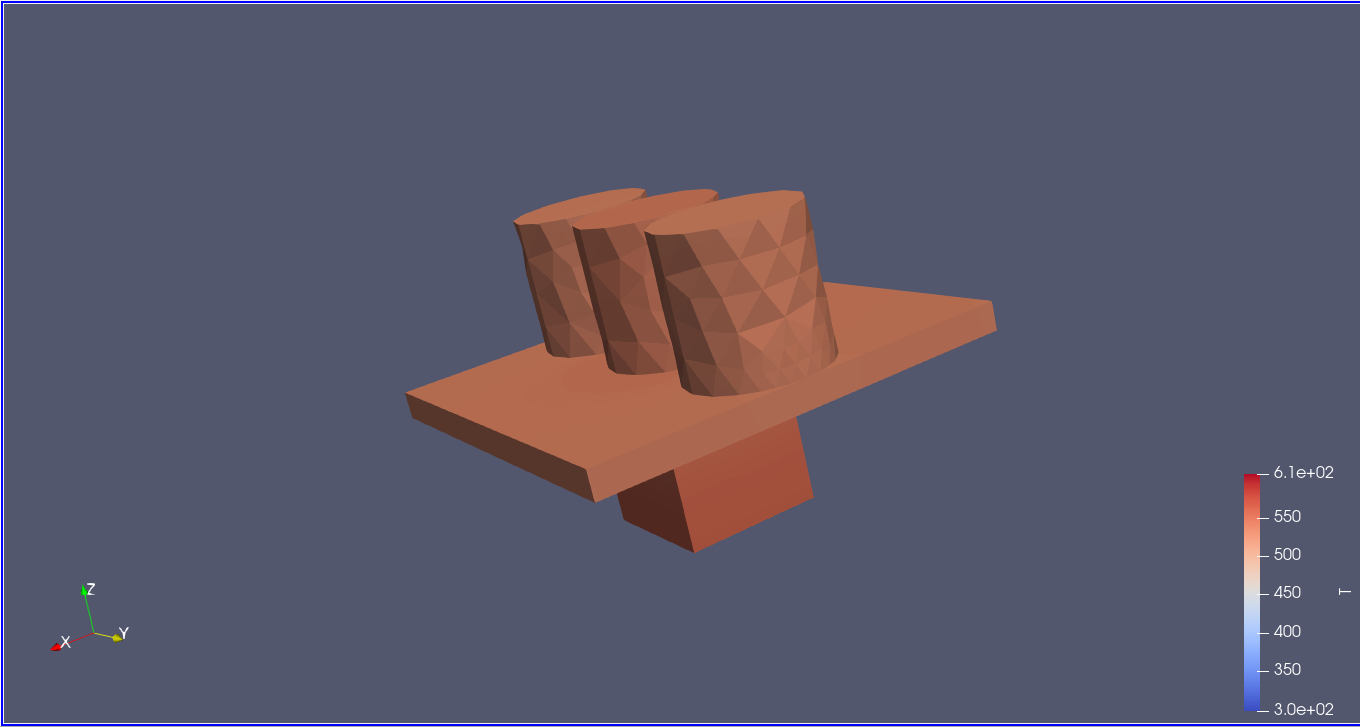
\includegraphics[width=0.45\linewidth]{images/5.3.png}
		\caption{Распределение температуры для модели 3} %% подпись к рисунку
	\end{center}
\end{figure}

\newpage
Были получены следующие результаты для моделей:
\begin{enumerate}
	\item \textbf{Первая модель:}
	      \begin{itemize}
		      \item Средняя температура радиатора: 508.381 К
		      \item Средняя температура нагревателя: 533.363 К
		      \item Средняя температура интерфейса между нагревателем и радиатором: 521.537 К
	      \end{itemize}
	\item \textbf{Вторая модель:}
	      \begin{itemize}
		      \item Средняя температура радиатора: 555.23 К
		      \item Средняя температура нагревателя: 576.306 К
		      \item Средняя температура интерфейса между нагревателем и радиатором: 564.451 К
	      \end{itemize}
	\item \textbf{Третья модель:}
	      \begin{itemize}
		      \item Средняя температура радиатора: 519.325 К
		      \item Средняя температура нагревателя: 537.741 К
		      \item Средняя температура интерфейса между нагревателем и радиатором: 525.862 К
	      \end{itemize}
\end{enumerate}

Построены графики температуры в нагревателе:
\newpage
\begin{figure}[h]
	\begin{center}
		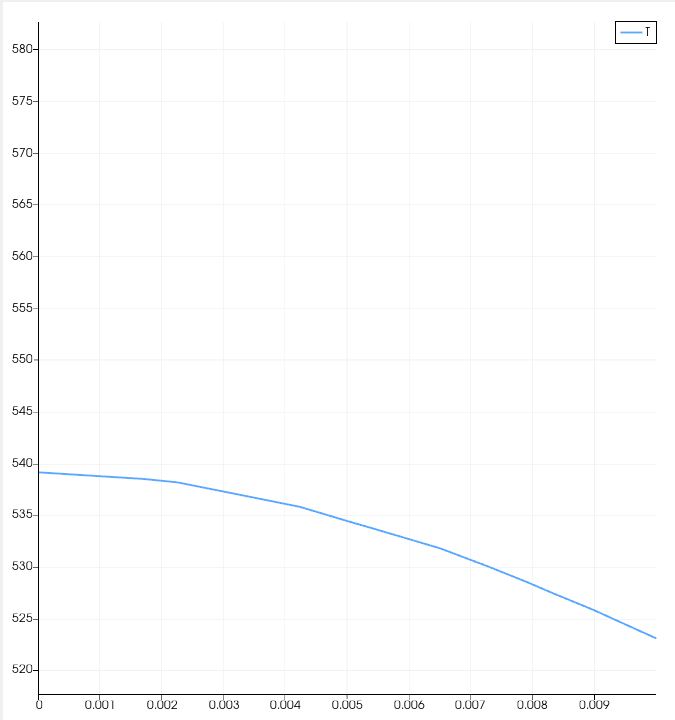
\includegraphics[width=0.4\linewidth]{images/6.1.png}
		\caption{Распределение температуры в нагревателе для модели 1} %% подпись к рисунку
	\end{center}
\end{figure}
\begin{figure}[h]
	\begin{center}
		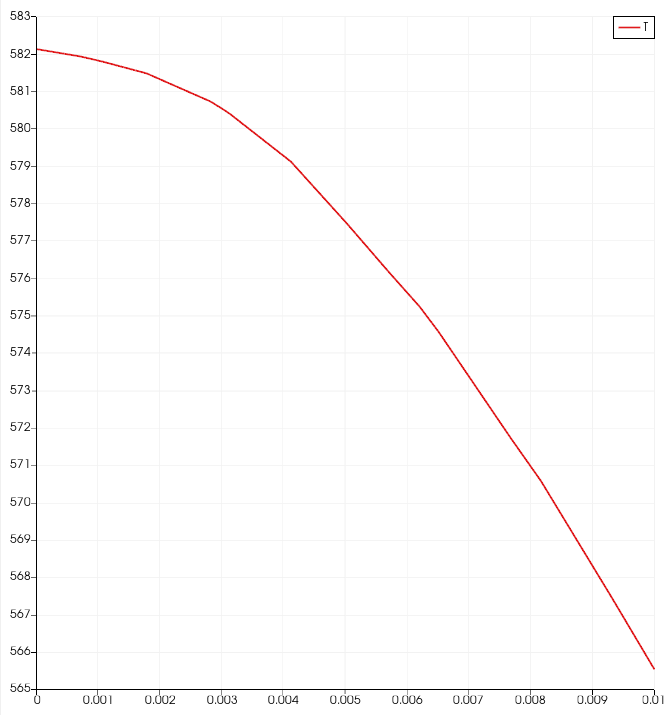
\includegraphics[width=0.4\linewidth]{images/6.2.png}
		\caption{Распределение температуры в нагревателе для модели 2} %% подпись к рисунку
	\end{center}
\end{figure}
\newpage
\begin{figure}[h]
	\begin{center}
		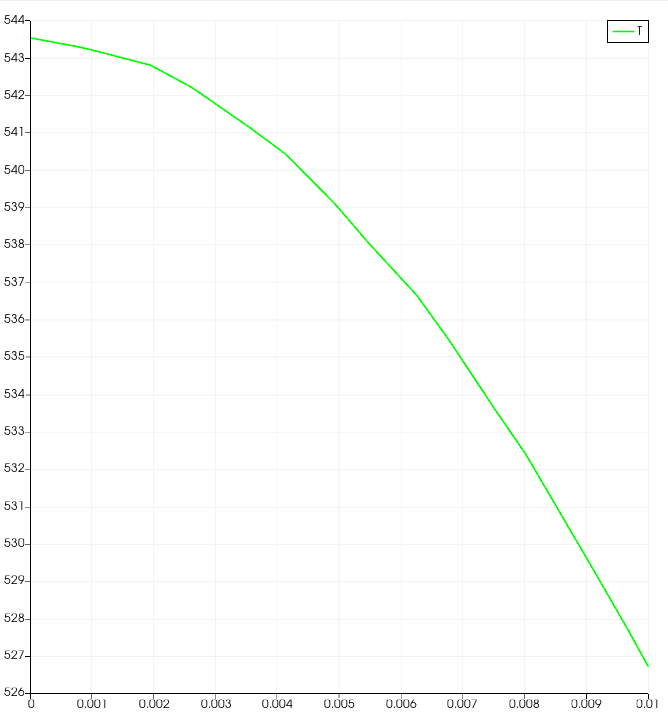
\includegraphics[width=0.4\linewidth]{images/6.3.png}
		\caption{Распределение температуры в нагревателе для модели 3} %% подпись к рисунку
	\end{center}
\end{figure}
\begin{figure}[h]
	\begin{center}
		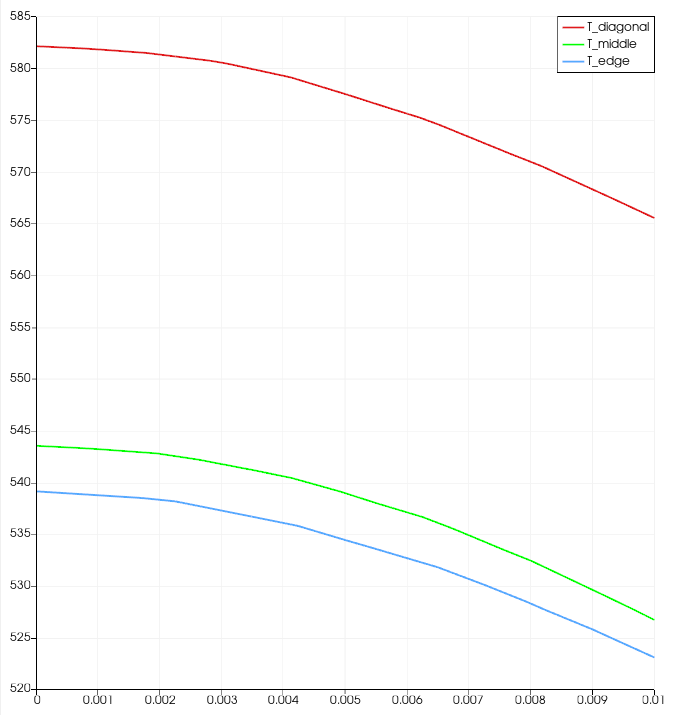
\includegraphics[width=0.4\linewidth]{images/6.png}
		\caption{Распределение температур в нагревателях для всех моделей} %% подпись к рисунку
	\end{center}
\end{figure}

\newpage
\par
Затем было проведено 2000 итераций расчета. Для отслеживания сходимости во время проведения расчета были построены следующие графики (пример для модели 1):
\begin{figure}[h]
	\begin{center}
		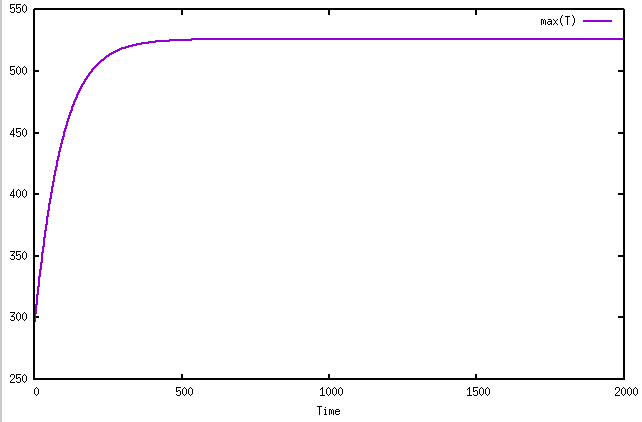
\includegraphics[width=0.35\linewidth]{images/11.1.png}
		\caption{Зависимость максимальной температуры радиатора от шага} %% подпись к рисунку
	\end{center}
\end{figure}
\begin{figure}[h]
	\begin{center}
		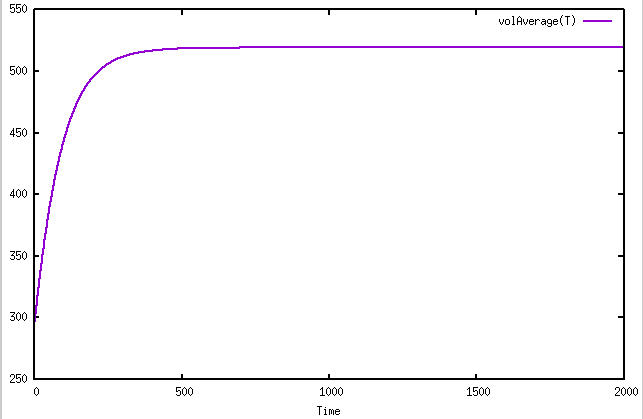
\includegraphics[width=0.35\linewidth]{images/12.1.png}
		\caption{Зависимость средней температуры радиатора от шага} %% подпись к рисунку
	\end{center}
\end{figure}
\begin{figure}[h]
	\begin{center}
		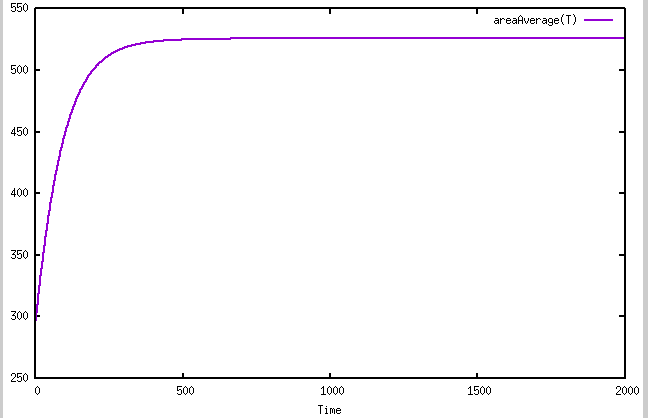
\includegraphics[width=0.35\linewidth]{images/13.1.png}
		\caption{Зависимость средней температуры интерфейса между нагревателем и радиатором от шага} %% подпись к рисунку
	\end{center}
\end{figure}
\newpage
\begin{figure}[h]
	\begin{center}
		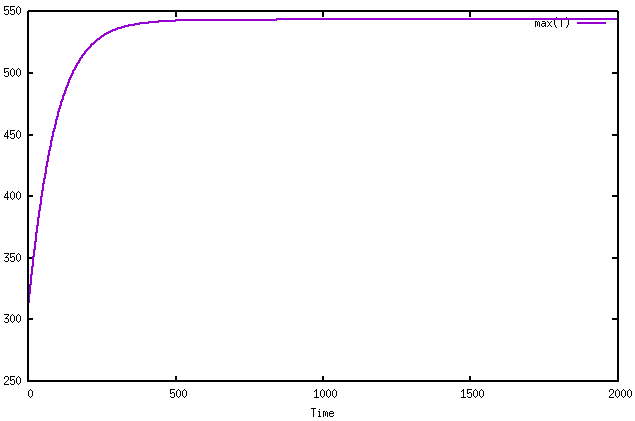
\includegraphics[width=0.4\linewidth]{images/14.1.png}
		\caption{Зависимость максимальной температуры нагревателя от шага} %% подпись к рисунку
	\end{center}
\end{figure}
\begin{figure}[h]
	\begin{center}
		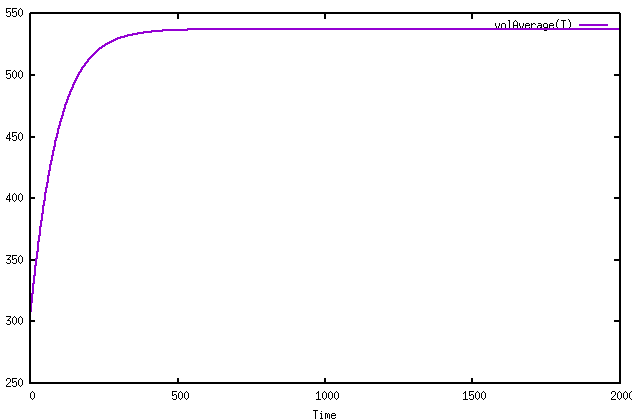
\includegraphics[width=0.4\linewidth]{images/15.1.png}
		\caption{Зависимость средней температуры нагревателя от шага} %% подпись к рисунку
	\end{center}
\end{figure}

\par
Далее были построены графики распределений температуры в центральном сечении:

\begin{figure}[h]
	\begin{center}
		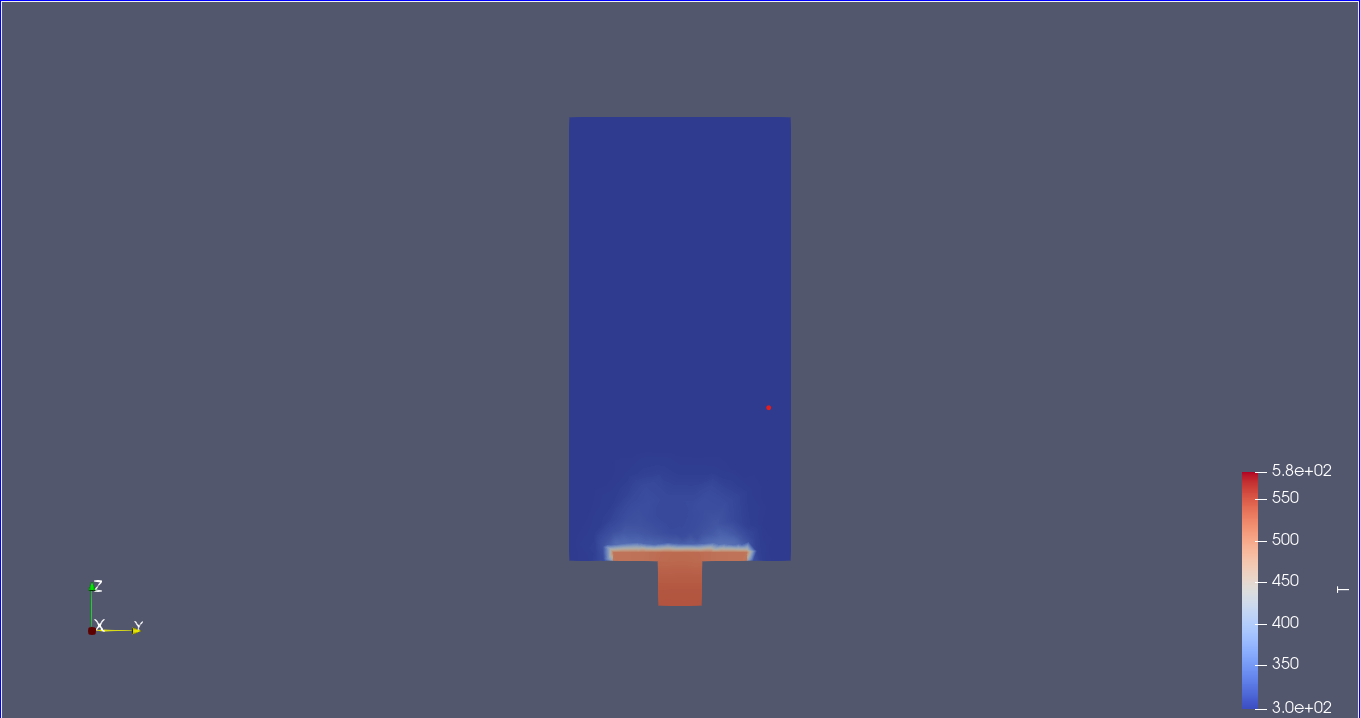
\includegraphics[width=0.4\linewidth]{images/7.1.png}
		\caption{Распределение температуры для модели 1} %% подпись к рисунку
	\end{center}
\end{figure}

\begin{figure}[h]
	\begin{center}
		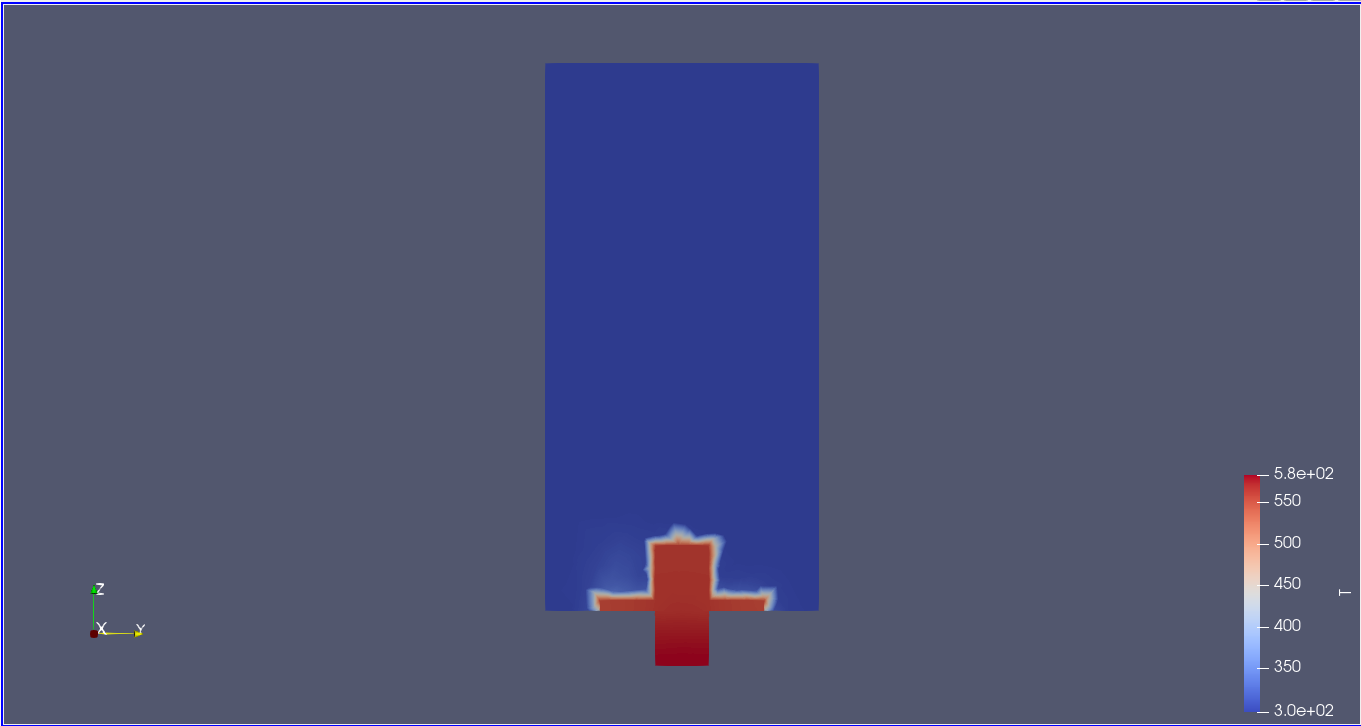
\includegraphics[width=0.4\linewidth]{images/7.2.png}
		\caption{Распределение температуры для модели 2} %% подпись к рисунку
	\end{center}
\end{figure}
\newpage
\begin{figure}[h]
	\begin{center}
		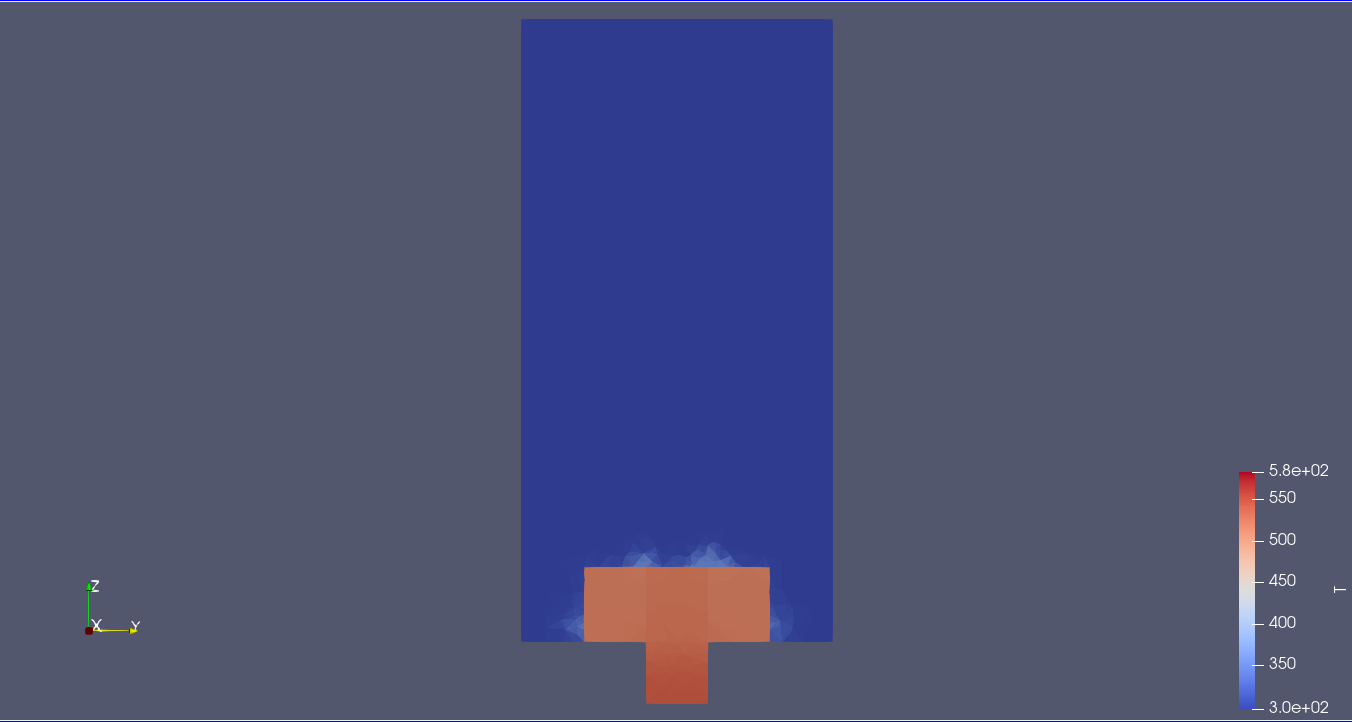
\includegraphics[width=0.4\linewidth]{images/7.3.png}
		\caption{Распределение температуры для модели 3} %% подпись к рисунку
	\end{center}
\end{figure}

\par
А также графики распределений скоростей:
\begin{figure}[h]
	\begin{center}
		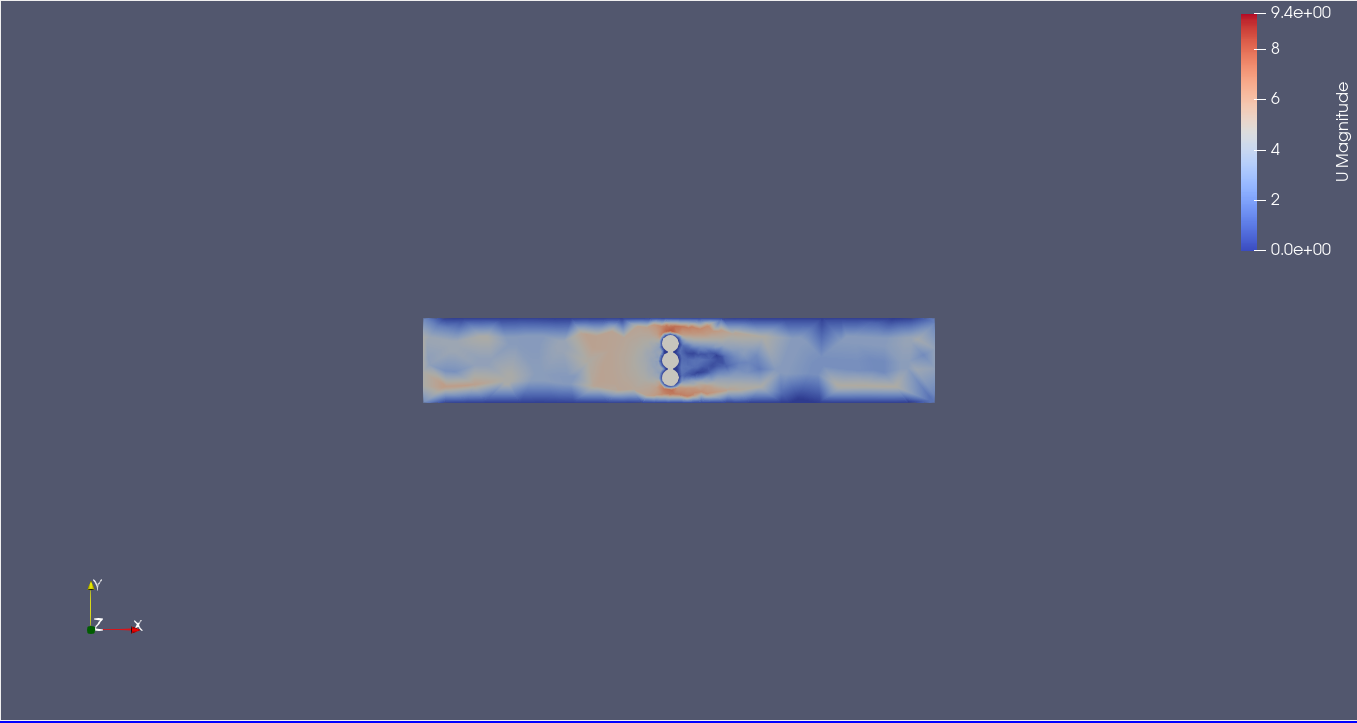
\includegraphics[width=0.4\linewidth]{images/8.1.png}
		\caption{Распределение скоростей для модели 1} %% подпись к рисунку
	\end{center}
\end{figure}

\begin{figure}[h]
	\begin{center}
		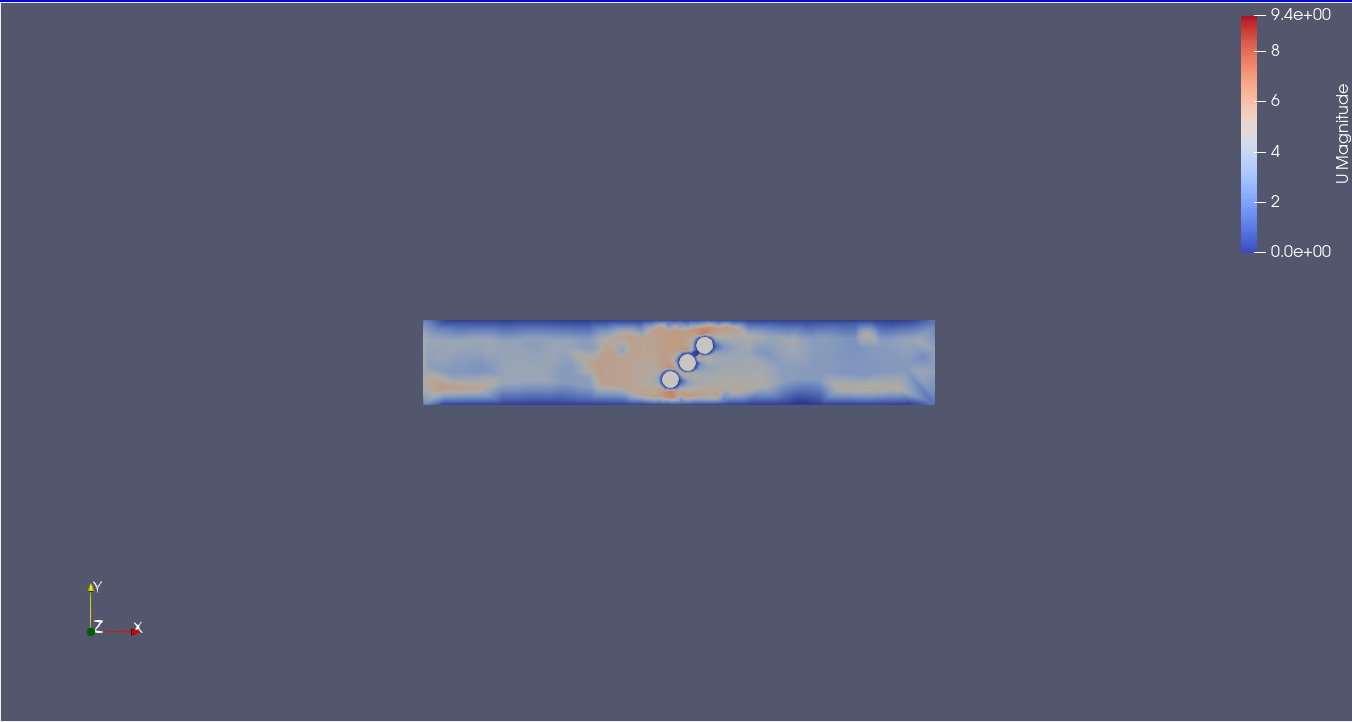
\includegraphics[width=0.4\linewidth]{images/8.2.png}
		\caption{Распределение скоростей для модели 2} %% подпись к рисунку
	\end{center}
\end{figure}
\newpage
\begin{figure}[h]
	\begin{center}
		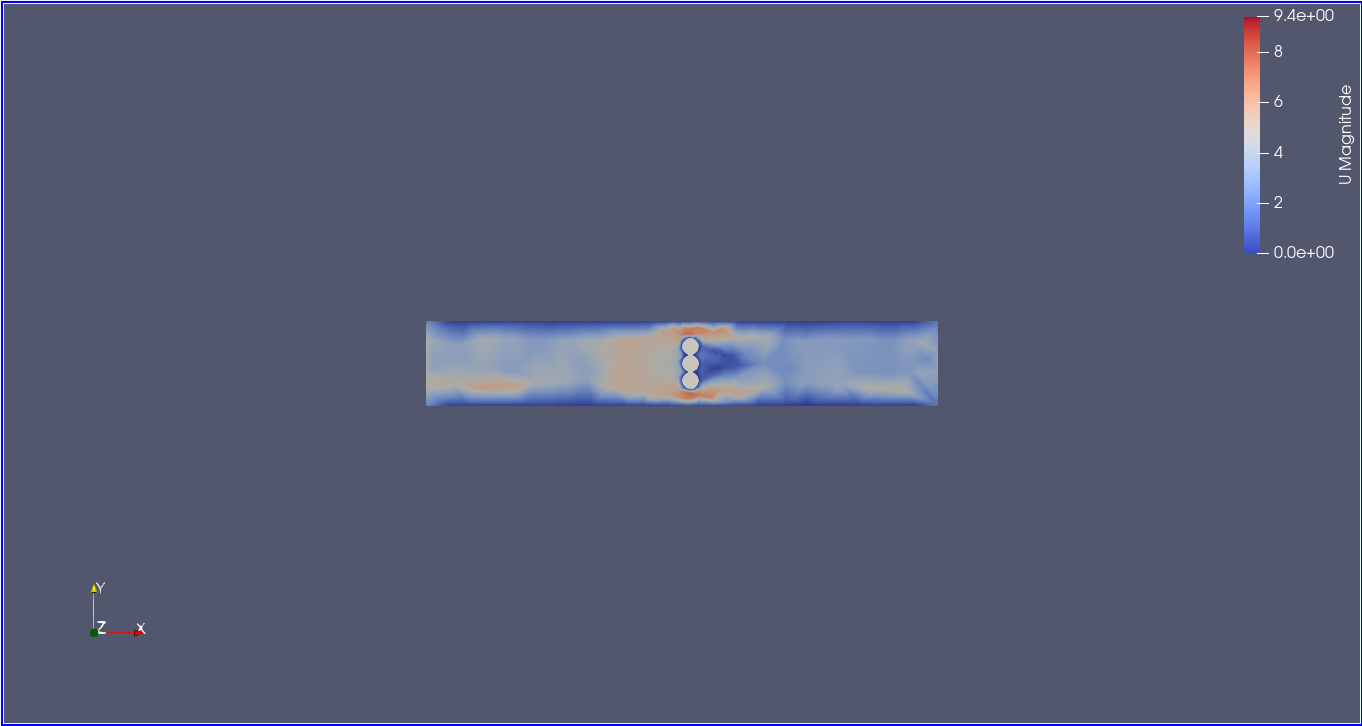
\includegraphics[width=0.4\linewidth]{images/8.3.png}
		\caption{Распределение скоростей для модели 3} %% подпись к рисунку
	\end{center}
\end{figure}
\begin{figure}[h]
	\begin{center}
		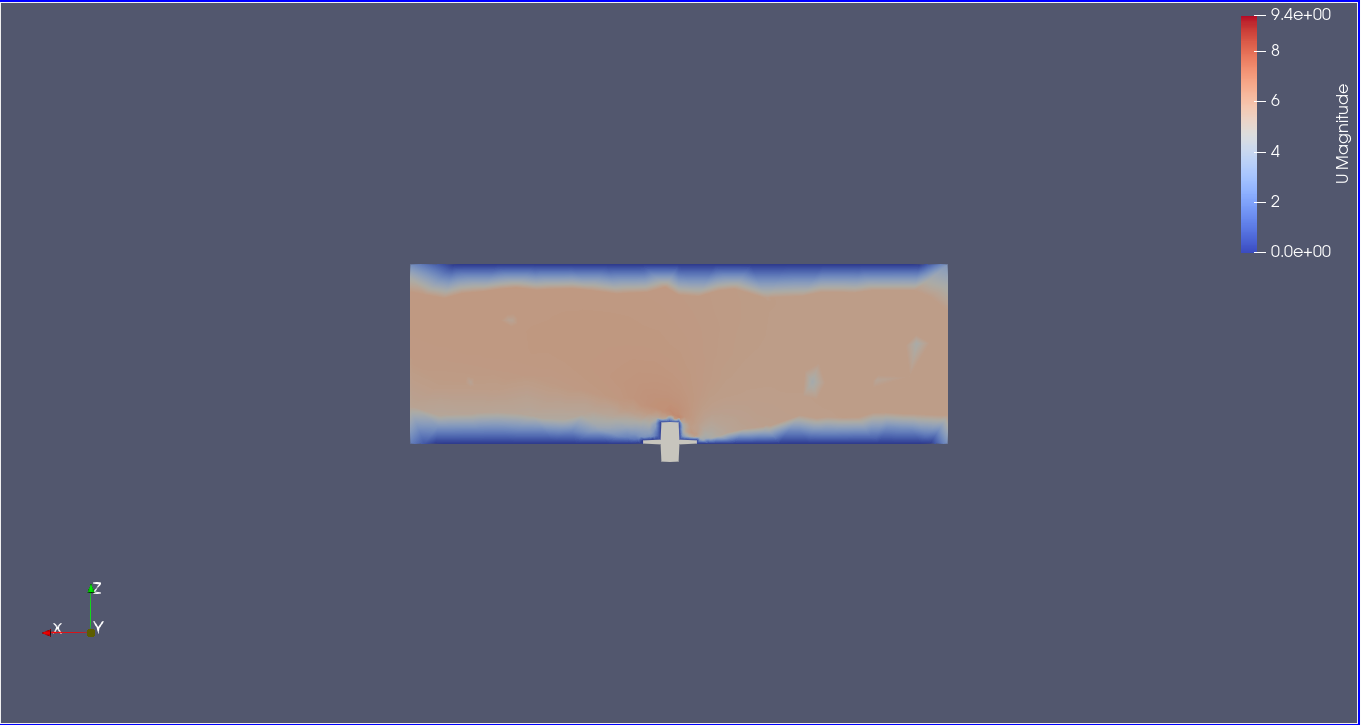
\includegraphics[width=0.4\linewidth]{images/9.png}
		\caption{Распределение скоростей для модели 1} %% подпись к рисунку
	\end{center}
\end{figure}

\section{Автоматическая генерация сетки в SALOME}

В ходе исследования при перегенерации геометрии в SALOME, задействовав дамп скрипта, была получена сетка с ошибками из-за нарушения идентификаторов (ID) сущностей.

Для решения данной проблемы был использован Python API в SALOME и применялись следующие методы:
\subsection{\texttt{SubShapeAllIDs}}

Функция \texttt{SubShapeAllIDs} в Python API SALOME используется для получения всех идентификаторов (ID) подформ в геометрии. Это полезно, когда необходимо провести операции с каждой подформой в модели.

Пример использования:
\begin{verbatim}
subshape_ids = geompy.SubShapeAllIDs(main_shape)
print(f"ID подформ: {subshape_ids}")
\end{verbatim}

В данном примере \texttt{main\_shape} - это главная форма в вашей геометрии.

\subsection{\texttt{GetShapesOnBoxIDs}}

Функция \texttt{GetShapesOnBoxIDs} возвращает идентификаторы форм, которые содержатся внутри заданного объема, определенного прямоугольным параллелепипедом.

Пример использования:
\begin{verbatim}
box = geompy.MakeBox(0, 0, 0, 10, 10, 10)
shapes_inside_box_ids = geompy.GetShapesOnBoxIDs(main_shape, box)
print(f"ID форм внутри прямоугольного параллелепипеда: {shapes_inside_box_ids}")
\end{verbatim}

Здесь \texttt{main\_shape} - это опять же главная форма, а \texttt{box} - созданный прямоугольный параллелепипед.

\subsection{\texttt{GetShapesOnPlaneWithLocationIDs}}

Функция \texttt{GetShapesOnPlaneWithLocationIDs} возвращает идентификаторы форм, которые пересекают заданную плоскость.

Пример использования:
\begin{verbatim}
plane = geompy.MakePlane(0, 0, 1, 0)
shapes_on_plane_ids = geompy.GetShapesOnPlaneWithLocationIDs(main_shape, plane)
print(f"ID форм, пересекаемых плоскостью: {shapes_on_plane_ids}")
\end{verbatim}

В этом примере \texttt{main\_shape} - главная форма, а \texttt{plane} - созданная плоскость \cite{salome_doc}.

Используя эти методы, получилось стабилизировать процесс генерации сетки, обеспечивая постоянство идентификаторов форм даже при обновлении геометрии. Это решение позволило успешно использовать скрипт в дальнейших этапах исследования.

\section{Автоматизированный пайплайн для генерации сетки, расчета и аналитики}

На данном этапе работы рассматривается процесс автоматизации генерации сетки в программе SALOME и выполнения расчетов в OpenFOAM для различных комбинаций параметров. Ключевыми параметрами, подлежащими варьированию, являются \\ \texttt{shift\_first\_cylinder} и \texttt{shift\_second\_cylinder}.

Переменная \texttt{shift\_first\_cylinder} представляет собой сдвиг первого цилиндра в радиаторе, а \texttt{shift\_second\_cylinder} — сдвиг второго цилиндра. Эти параметры влияют на геометрию радиатора и, следовательно, на условия теплообмена в системе.

Скрипт создает уникальное имя для каждой комбинации параметров и затем копирует исходный кейс в новую директорию. После этого SALOME запускается в режиме командной строки для выполнения генерации сетки с учетом новой геометрии, заданной параметрами сдвига цилиндров. Далее запускаются соответствующие bash-скрипты для выполнения кейса в OpenFOAM.

После завершения расчета, автоматически извлекаются результаты. Сценарий ищет и анализирует файл с данными теплообмена в постпроцессинговой директории. Это позволяет собирать и систематизировать конечные результаты для каждой конфигурации геометрии. Такой подход обеспечивает эффективный анализ влияния различных параметров на теплоотдачу системы.

\section{Особенности фиксации и движения цилиндров}

Необходимо отметить, что в проведенных исследованиях имелось три цилиндра в системе. Тем не менее, третий цилиндр был зафиксирован в положении (0, 0), и двигались только два оставшихся цилиндра. Такой выбор сделан с целью упростить визуализацию и анализ результатов.

Данный подход облегчает анализ и интерпретацию результатов, обеспечивая более ясное представление о влиянии конкретных параметров на эффективность теплообмена в рассматриваемой системе.

\section{Первые результаты}

На основе автоматизированного процесса получены результаты, охватывающие 25 точек варьирования параметров. Исследуемые параметры \texttt{shift\_first\_cylinder} и \texttt{shift\_second\_cylinder} изменялись от 0 мм до 20 мм с шагом 5 мм.
Эти значения представляют различные комбинации сдвигов цилиндров в радиаторе, что отражает влияние геометрических параметров на теплоотдачу системы.

\begin{figure}[h]
	\begin{center}
		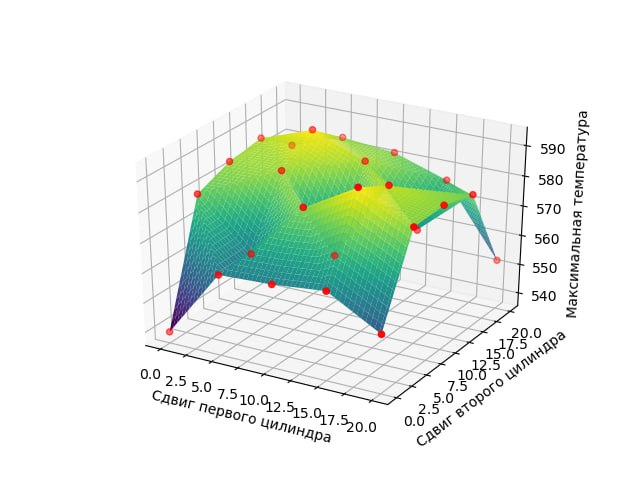
\includegraphics[width=0.4\linewidth]{images/16.1.jpg}
		\caption{Зависимость максимальной температуры нагревателя от сдвигов цилиндров} %% подпись к рисунку
	\end{center}
\end{figure}

\begin{figure}[h]
	\begin{center}
		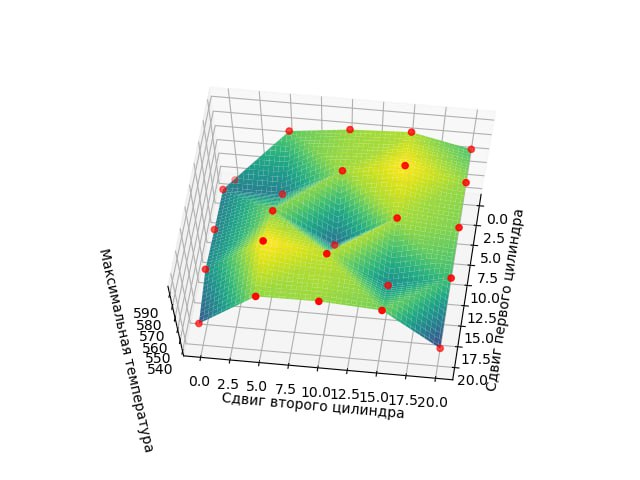
\includegraphics[width=0.4\linewidth]{images/16.2.jpg}
		\caption{Зависимость максимальной температуры нагревателя от сдвигов цилиндров} %% подпись к рисунку
	\end{center}
\end{figure}
\newpage
\begin{figure}[h]
	\begin{center}
		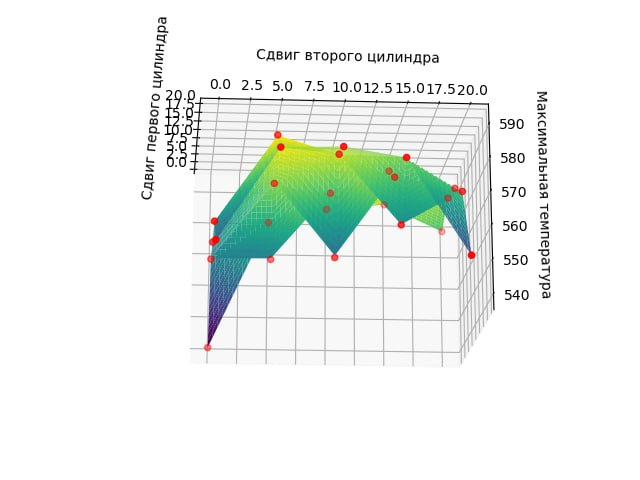
\includegraphics[width=0.4\linewidth]{images/16.3.jpg}
		\caption{Зависимость максимальной температуры нагревателя от сдвигов цилиндров} %% подпись к рисунку
	\end{center}
\end{figure}

Для улучшения визуализации и наглядности полученных данных была проведена интерполяция поверхности.
Интерполированная поверхность дает представление о поведении системы в пространстве параметров и позволяет выявить области оптимальных значений для исследуемых параметров.
Этот этап анализа предоставляет первичное представление о влиянии сдвига цилиндров на теплообмен в системе.

\section{Оптимизация процесса расчета}

Для оптимизации расчета множества точек был создан многопроцессорный код на языке программирования Python. 
Данное решение позволяет эффективно использовать ресурсы современных многоядерных процессоров, распределяя задачи между процессами и выполняя их параллельно.
Многопроцессорный подход обеспечивает лучшую производительность и масштабируемость по сравнению с многопоточностью, так как процессы работают в отдельных адресных пространствах и не делят общую память, что избавляет от проблем синхронизации и блокировок.
Реализация выполнена с помощью модуля multiprocessing. Ключевая функция run_simulation выполняет расчет для каждого набора параметров в отдельном процессе.
Она принимает уникальный идентификатор набора параметров и сами параметры, выполняет вычисления и возвращает результат.
Результаты сохраняются в разделяемом словаре all_data, где ключами выступают уникальные идентификаторы комбинаций параметров, например, _0_0_0, а значениями — результаты расчетов.
Разделяемый словарь all_data создан с использованием класса multiprocessing.Manager, который обеспечивает безопасный доступ к общим данным из разных процессов.
Для обработки различных комбинаций параметров используется класс multiprocessing.Pool и метод starmap. Этот метод принимает на вход функцию run_simulation и список аргументов в виде кортежей, содержащих уникальные идентификаторы и значения параметров.
Pool автоматически распределяет задачи между процессами и управляет их выполнением.
Параметризация количества процессов при создании экземпляра Pool позволяет настроить уровень параллелизма в зависимости от доступных ресурсов.
После завершения всех процессов, результаты собираются в разделяемом словаре all_data.
Этот словарь можно использовать для дальнейшего анализа, построения интерполяций или других задач, требующих доступа к полученным данным.
Применение многопроцессорности в Python значительно ускоряет вычисления, особенно при большом числе комбинаций параметров для анализа.
Распараллеливание вычислений на несколько процессов эффективно использует вычислительные ресурсы и позволяет обрабатывать большие объемы данных за меньшее время.
Это особенно важно для ресурсоемких задач, таких как оптимизация, параметрические исследования или анализ чувствительности.

\section{Увеличение количества точек для анализа}

Оптимизация процесса расчета с использованием многопоточности значительно повысила эффективность анализа.

Так, на следующем этапе было проведено исследование с шагом 2, что дало 121 точку для анализа.
Это уже более подробное и детальное исследование, которое позволяет получить более точные представления о влиянии параметров на характеристики системы.

\begin{figure}[h]
	\begin{center}
		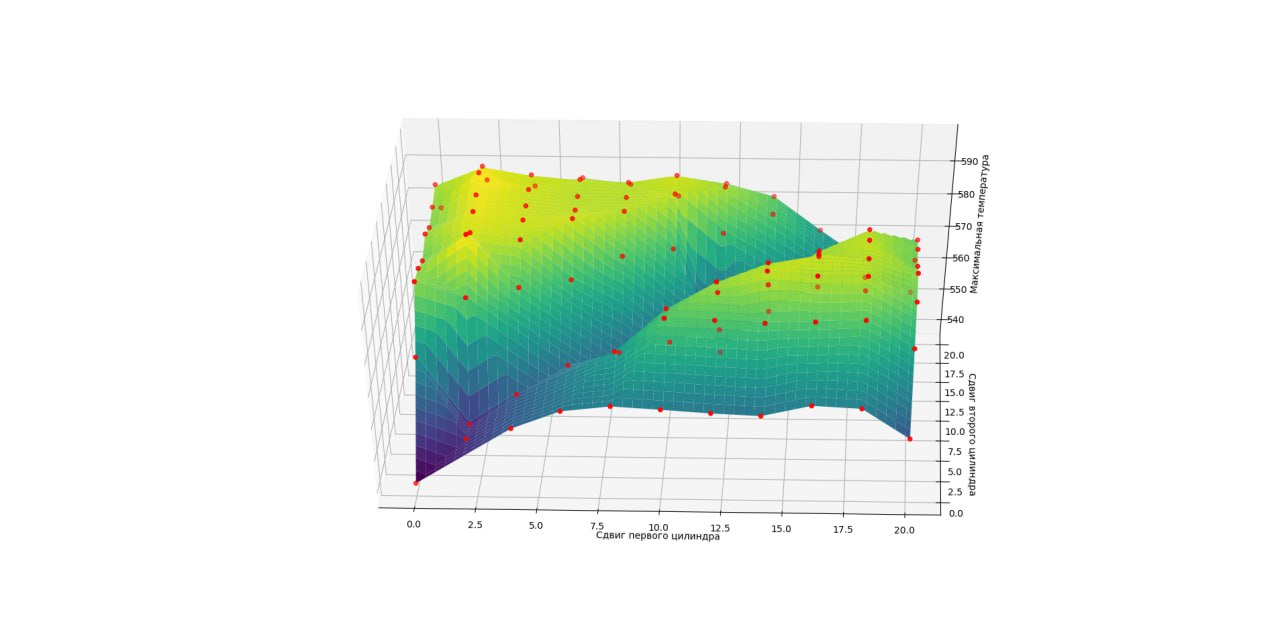
\includegraphics[width=0.4\linewidth]{images/17.1.jpg}
		\caption{Зависимость максимальной температуры нагревателя от сдвигов цилиндров (121 точка)} %% подпись к рисунку
	\end{center}
\end{figure}
\begin{figure}[h]
	\begin{center}
		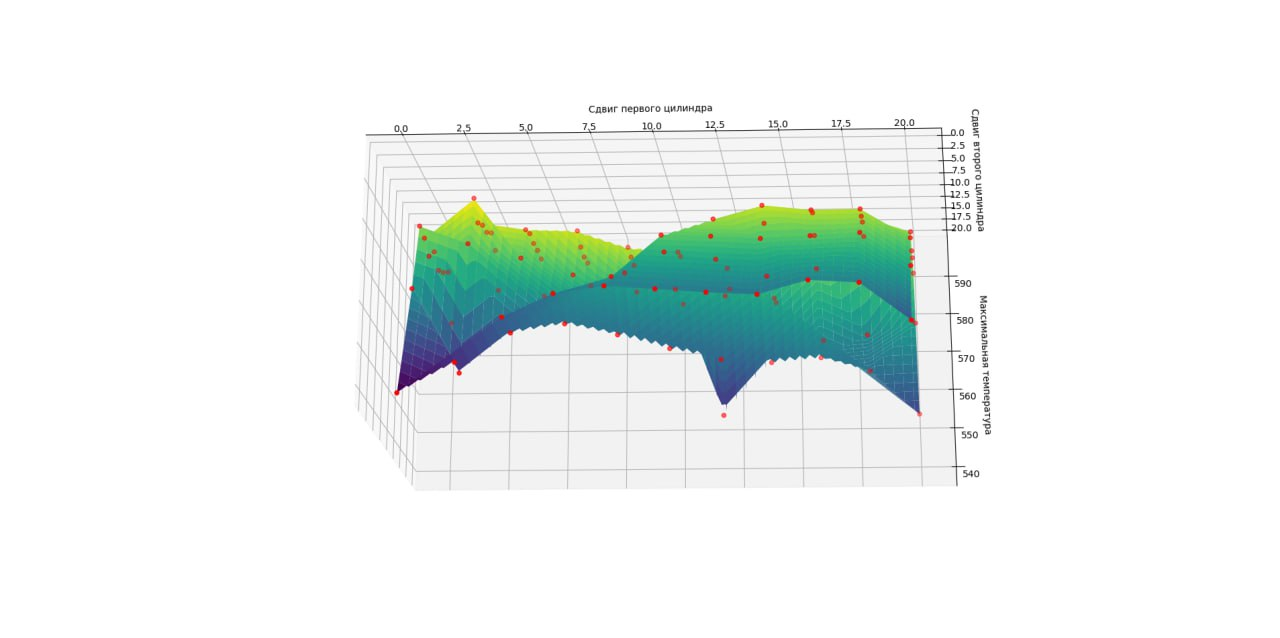
\includegraphics[width=0.4\linewidth]{images/17.2.jpg}
		\caption{Зависимость максимальной температуры нагревателя от сдвигов цилиндров (121 точка)} %% подпись к рисунку
	\end{center}
\end{figure}

Затем мы перешли к шагу 1, что привело к анализу 441 точки.

\begin{figure}[h]
	\begin{center}
		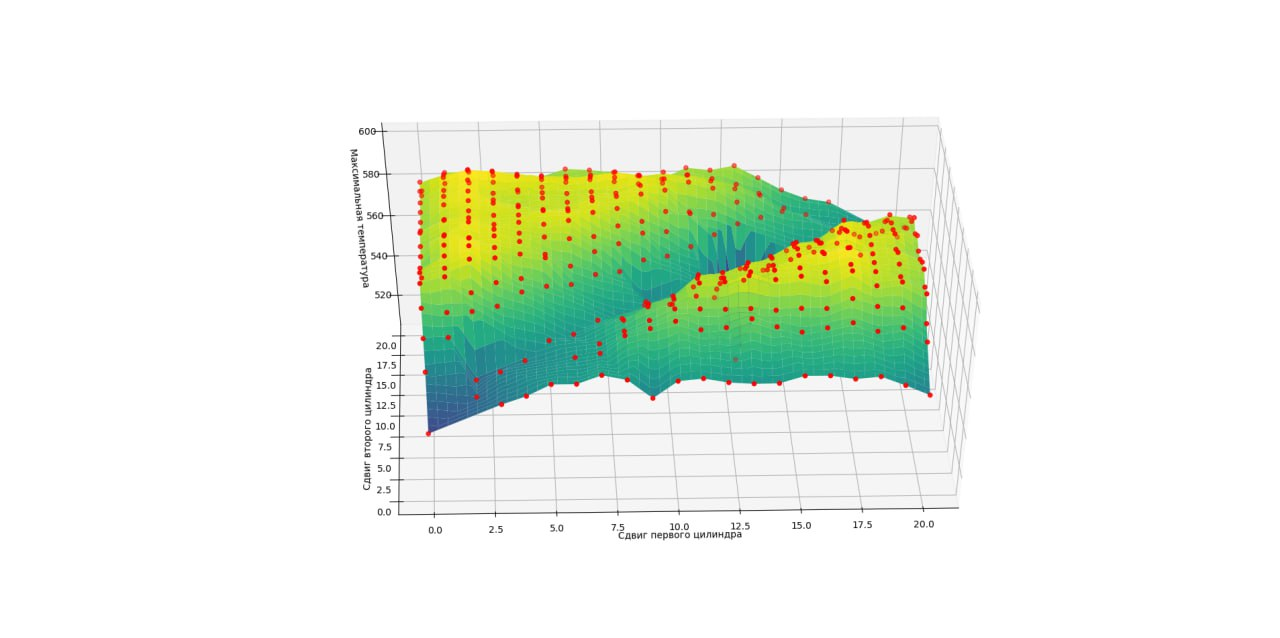
\includegraphics[width=0.4\linewidth]{images/18.1.jpg}
		\caption{Зависимость максимальной температуры нагревателя от сдвигов цилиндров (441 точка)} %% подпись к рисунку
	\end{center}
\end{figure}
\begin{figure}[h]
	\begin{center}
		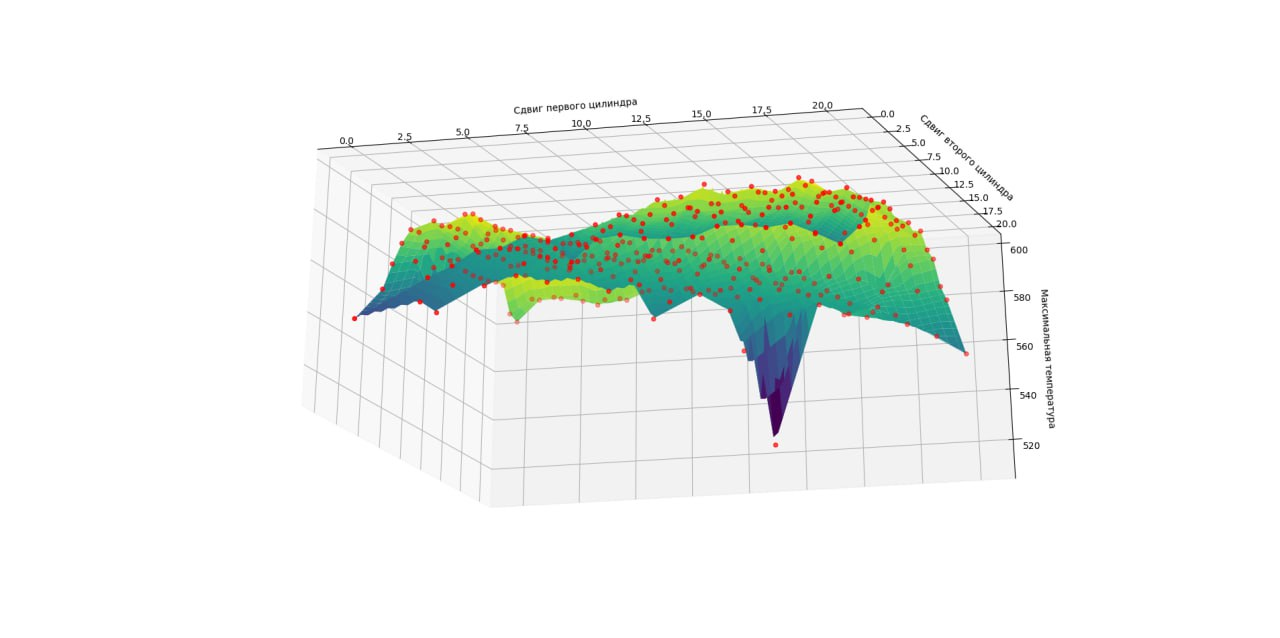
\includegraphics[width=0.4\linewidth]{images/18.2.jpg}
		\caption{Зависимость максимальной температуры нагревателя от сдвигов цилиндров (441 точка)} %% подпись к рисунку
	\end{center}
\end{figure}

\section{Результаты и наблюдения автоматической генерации и переборов вариантов}

Первые результаты анализа геометрии системы показали интересные закономерности. В частности, было отмечено, что минимумы характеристик системы наблюдаются при равных сдвигах первого и второго цилиндров.

\begin{figure}[h]
	\begin{center}
		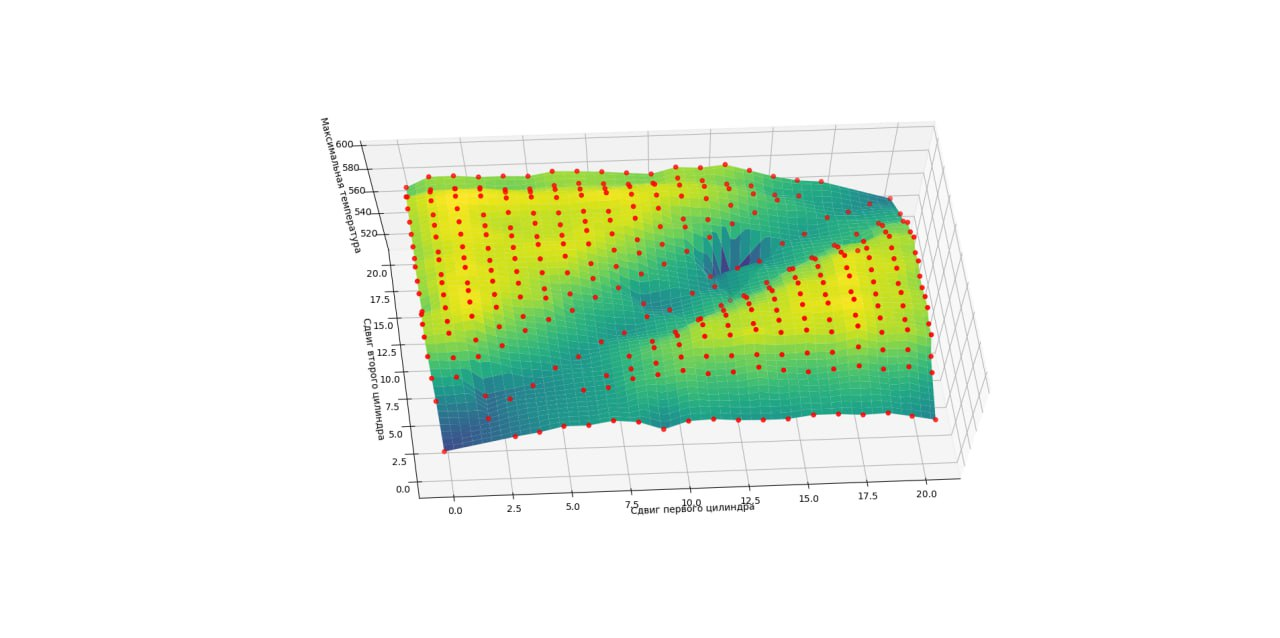
\includegraphics[width=0.4\linewidth]{images/18.3.jpg}
		\caption{Зависимость максимальной температуры нагревателя от сдвигов цилиндров (441 точка)} %% подпись к рисунку
	\end{center}
\end{figure}

При равных сдвигах цилиндров они касаются друг друга. Такая конфигурация способствует более эффективному теплообмену между цилиндрами и более равномерному распределению тепловой нагрузки.

\begin{figure}[h]
	\begin{center}
		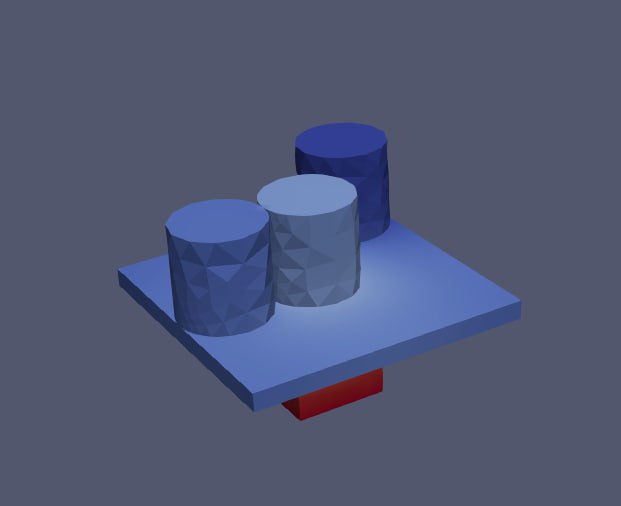
\includegraphics[width=0.4\linewidth]{images/19.jpg}
		\caption{Геометрия при которой достигается минимальное значение} %% подпись к рисунку
	\end{center}
\end{figure}

\section{Эксперименты с геометрией и анализ результатов}

Однако эта геометрия не демонстрировала реальной зависимости между расположением цилиндров и температурой. В ответ на это наблюдение был проведен ряд экспериментов с общей геометрией системы.

В первом эксперименте было решено уменьшить диаметр цилиндров в два раза, сделав их тоньше (2.5 мм). Это привело к тому, что цилиндры перестали касаться друг друга, создавая новые условия для теплообмена. Теперь теплообмен между цилиндрами осуществляется через воздушный зазор.

\begin{figure}[h]
	\begin{center}
		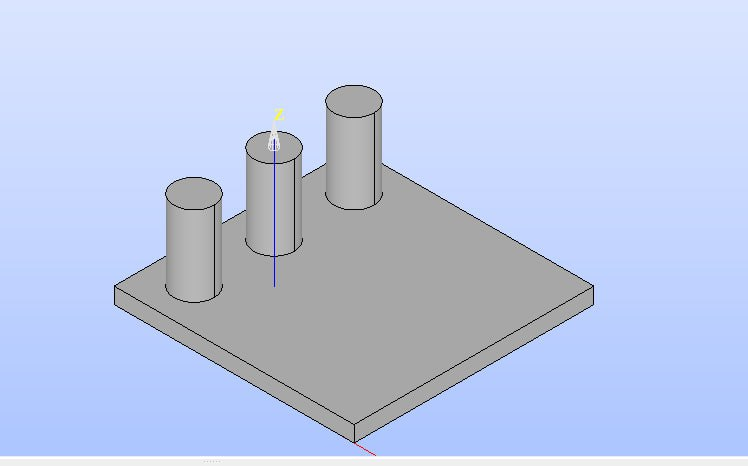
\includegraphics[width=0.4\linewidth]{images/20.jpg}
		\caption{Новая геометрия} %% подпись к рисунку
	\end{center}
\end{figure}

После внесения изменений в геометрию системы были получены более интересные результаты, которые отличаются от предыдущих экспериментов. Новая конфигурация цилиндров более чувствительна к расположению внутри системы, и температурные различия стали более заметными.

Например, можно заметить, что при размещении ближе к центру системы температуры становятся меньше. Это может быть обусловлено более равномерным распределением тепла в системе и более эффективным теплообменом.

\begin{figure}[h]
	\begin{center}
		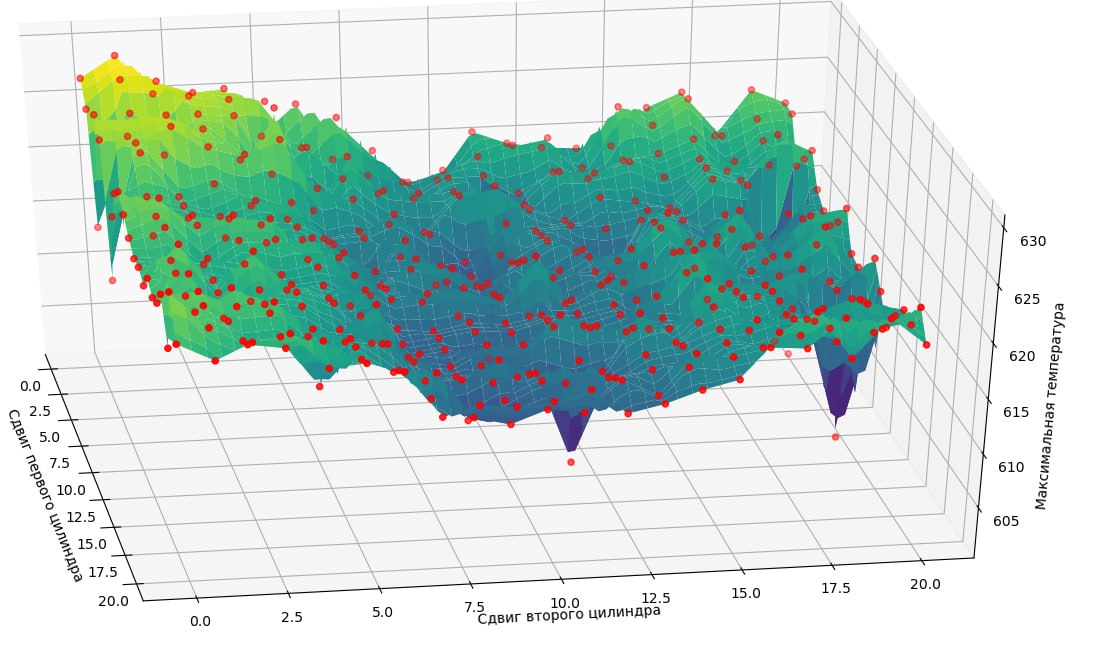
\includegraphics[width=0.4\linewidth]{images/21.1.jpg}
		\caption{Зависимость максимальной температуры нагревателя от сдвигов цилиндров} %% подпись к рисунку
	\end{center}
\end{figure}
\begin{figure}[h]
	\begin{center}
		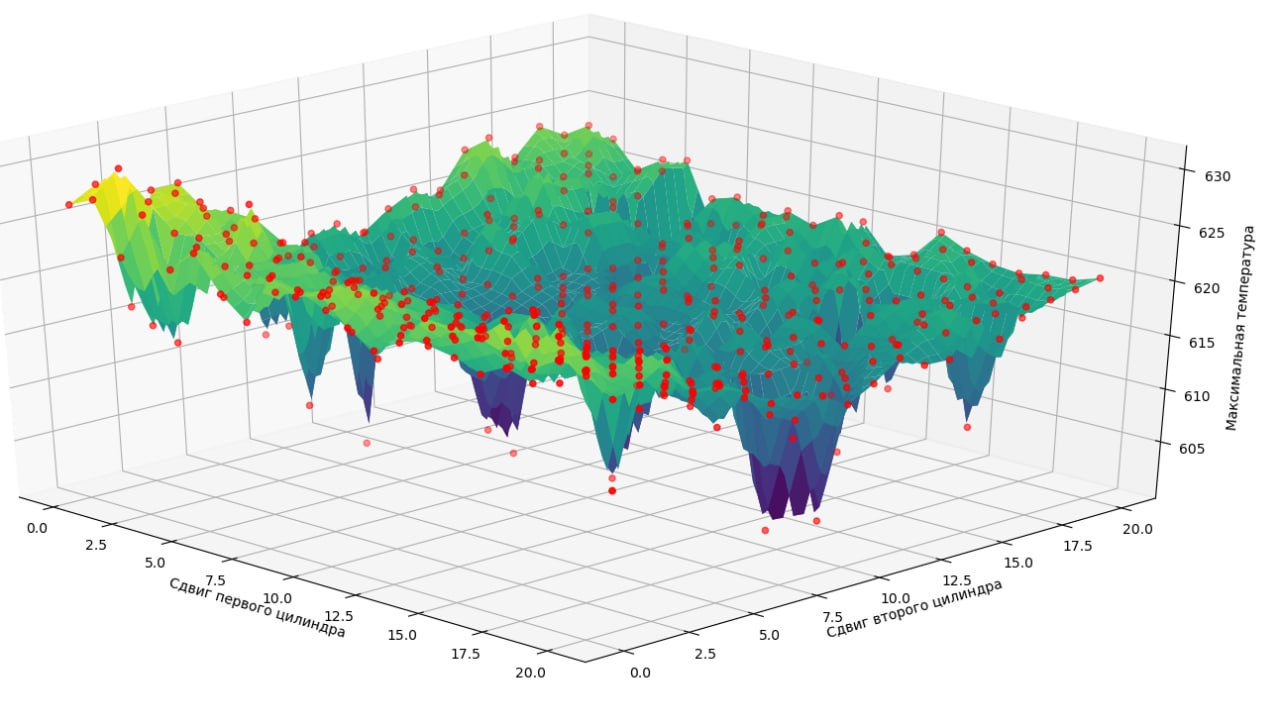
\includegraphics[width=0.4\linewidth]{images/21.2.jpg}
		\caption{Зависимость максимальной температуры нагревателя от сдвигов цилиндров} %% подпись к рисунку
	\end{center}
\end{figure}
\begin{figure}[h]
	\begin{center}
		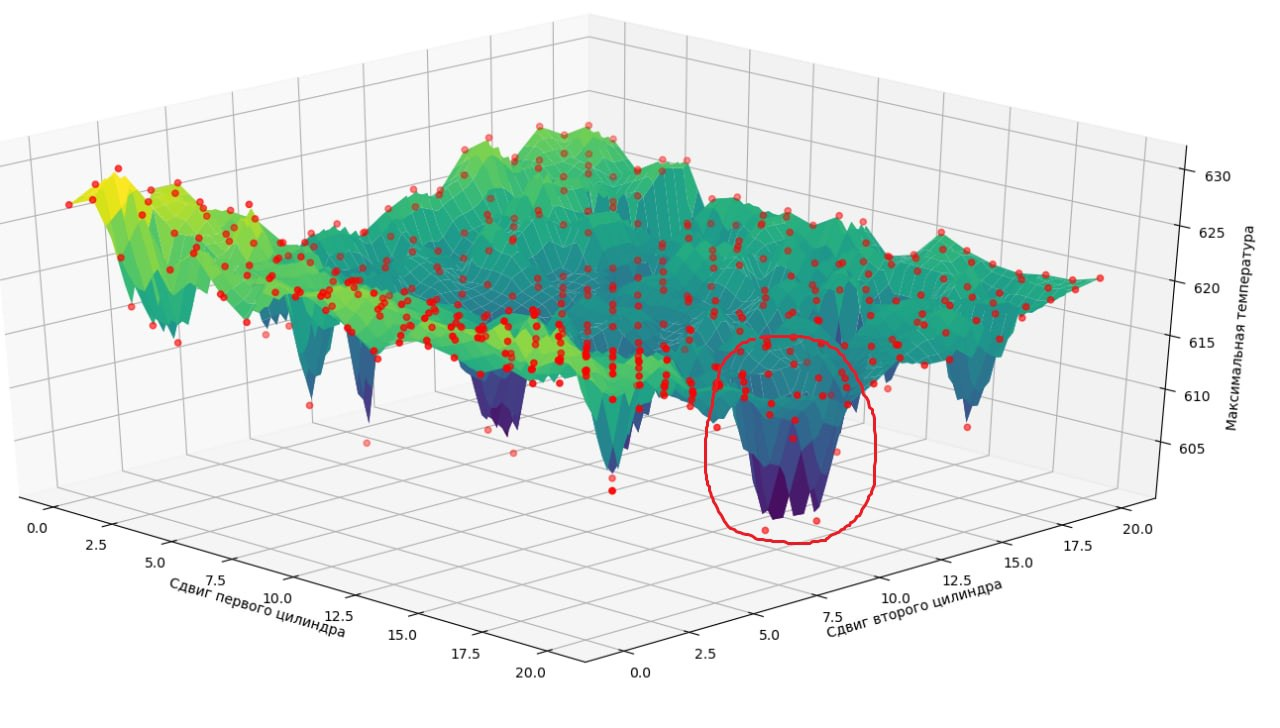
\includegraphics[width=0.4\linewidth]{images/21.3.jpg}
		\caption{Зависимость максимальной температуры нагревателя от сдвигов цилиндров} %% подпись к рисунку
	\end{center}
\end{figure}

В ходе экспериментов было обнаружено, что существует оптимальная конфигурация, при которой достигается минимум температуры в системе. Эта конфигурация характеризуется расстановкой цилиндров по диагонали (рис. 38 и 39). Минимум максимальной температуры нагревателя достигается также при данной конфигурации (рис. 40 и 41).

\begin{figure}[h]
	\begin{center}
		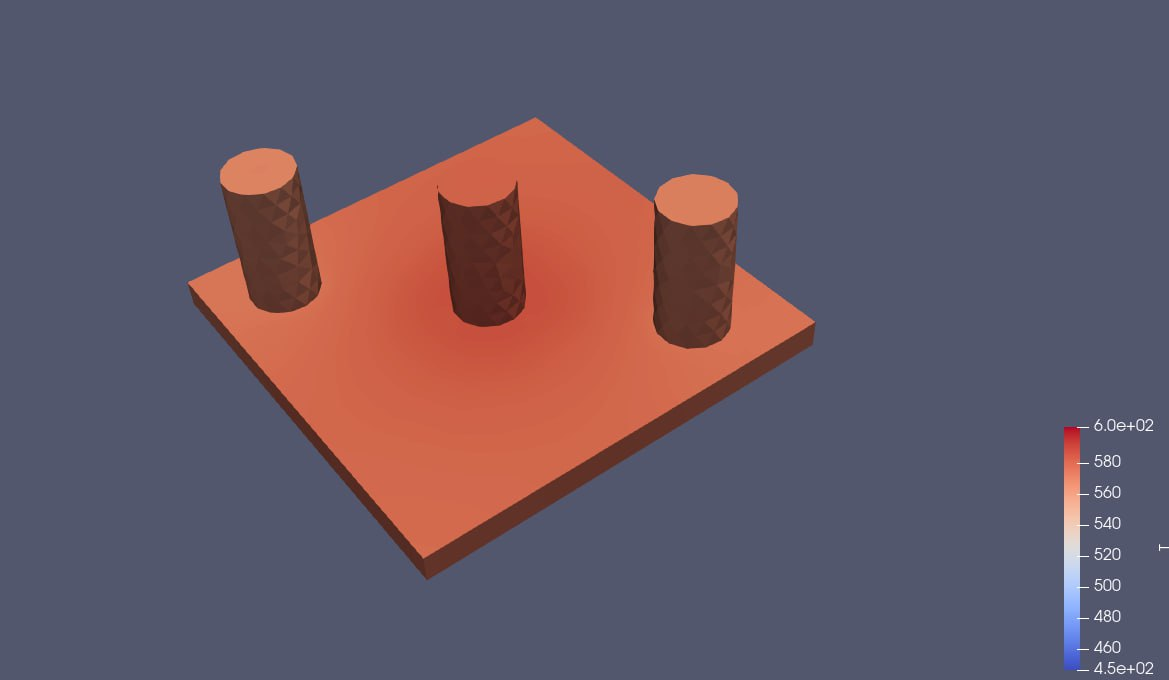
\includegraphics[width=0.4\linewidth]{images/21.4.jpg}
		\caption{Пример минимума при новой геометрии} %% подпись к рисунку
	\end{center}
\end{figure}

\newpage


\begin{figure}[h]
	\begin{center}
		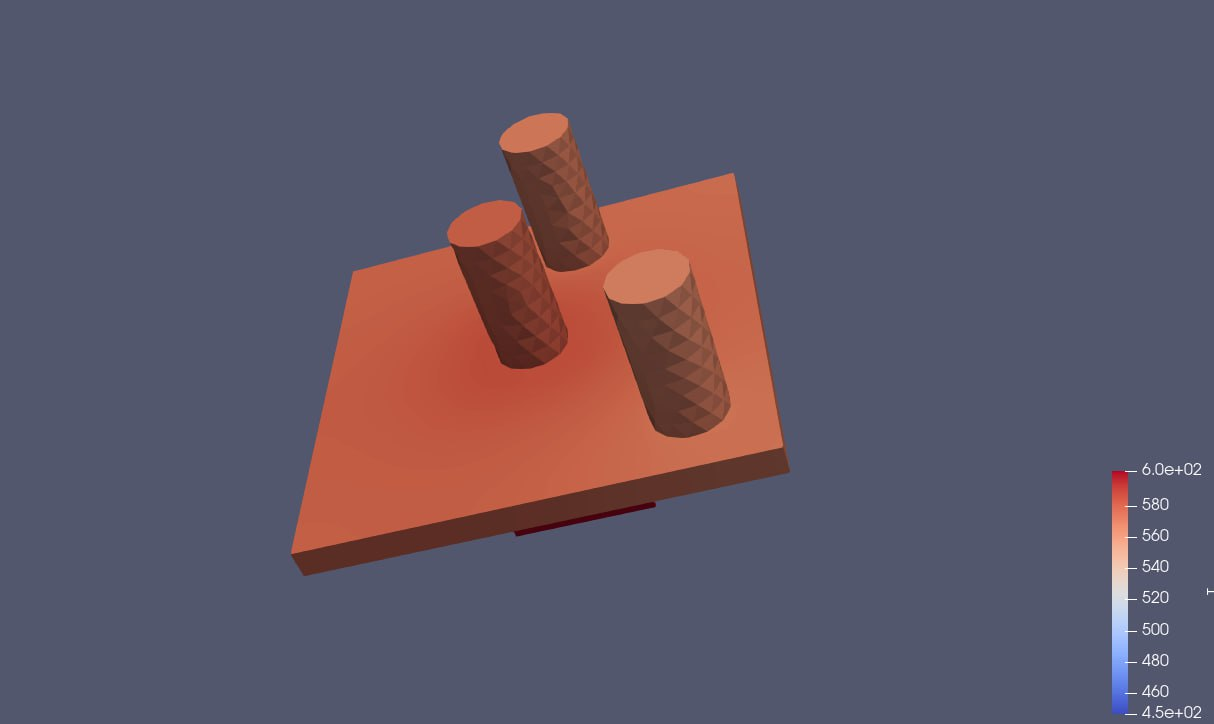
\includegraphics[width=0.4\linewidth]{images/21.5.jpg}
		\caption{Пример минимума при новой геометрии} %% подпись к рисунку
	\end{center}
\end{figure}

\section{Оптимизация расчетной сетки}

Для более глубокого анализа системы и выявления потенциальных выбросов в температурных данных, было решено оптимизировать расчетную сетку. Используя параметры NETGEN\_3D, уменьшен размер элементов сетки.

Этот подход позволил более детально рассмотреть поведение системы в местах с высокими градиентами температуры и выделить потенциальные выбросы. Результаты показали, что некоторые точки действительно являются выбросами, это может быть связано с особенностями теплового распределения в этих областях.

\section{Модификация геометрии и уменьшение воздуховода}

Далее была проведена серия изменений в геометрии системы. Одним из ключевых моментов стало уменьшение воздуховода практически до минимального зазора в 2 мм к цилиндрам. Это решение позволило избежать дополнительных условий на границе между воздуховодом и цилиндрами, создавая более естественные условия для теплового обмена.

С учетом внесенных изменений в геометрию системы и уменьшения воздуховода, проведен новый ряд расчетов и получены результаты, отраженные на рисунках 42 и 43.

\begin{figure}[h]
	\begin{center}
		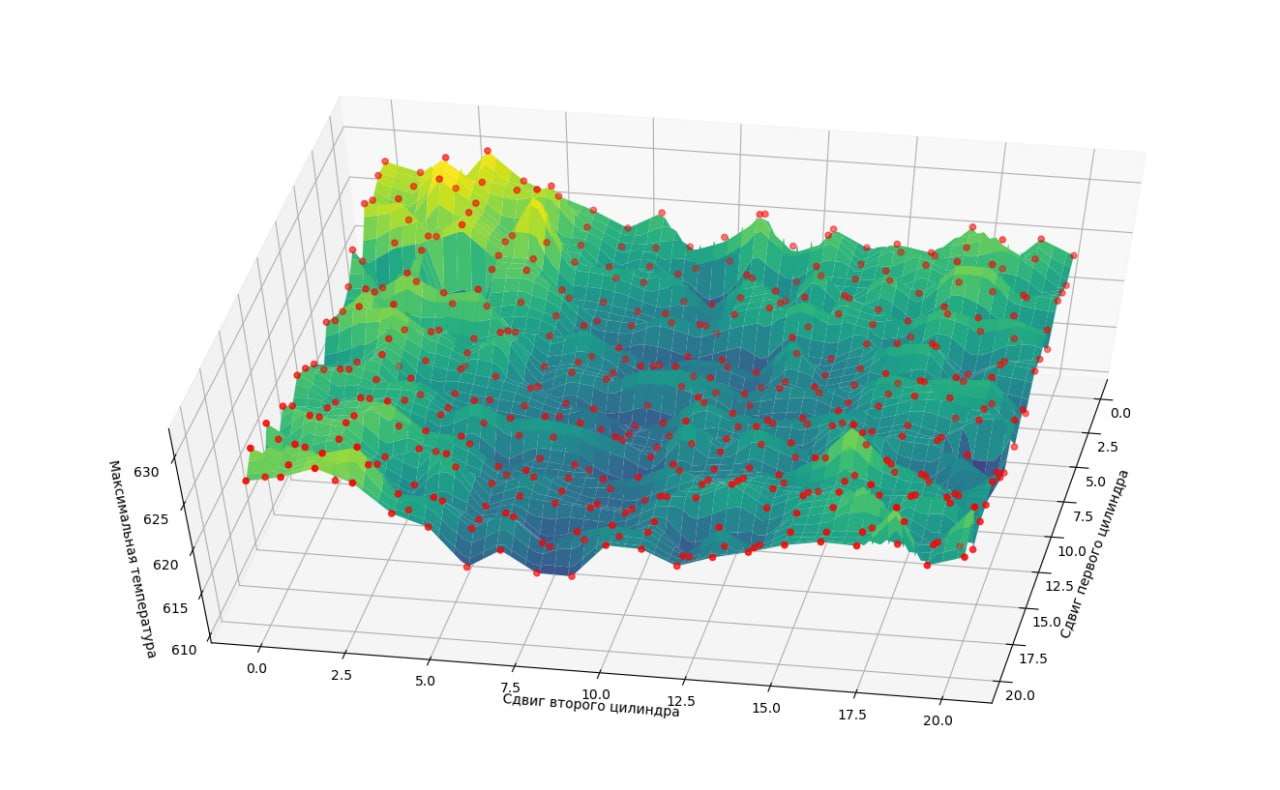
\includegraphics[width=0.4\linewidth]{images/22.1.jpg}
		\caption{Зависимость максимальной температуры нагревателя от сдвигов цилиндров} %% подпись к рисунку
	\end{center}
\end{figure}
\begin{figure}[h]
	\begin{center}
		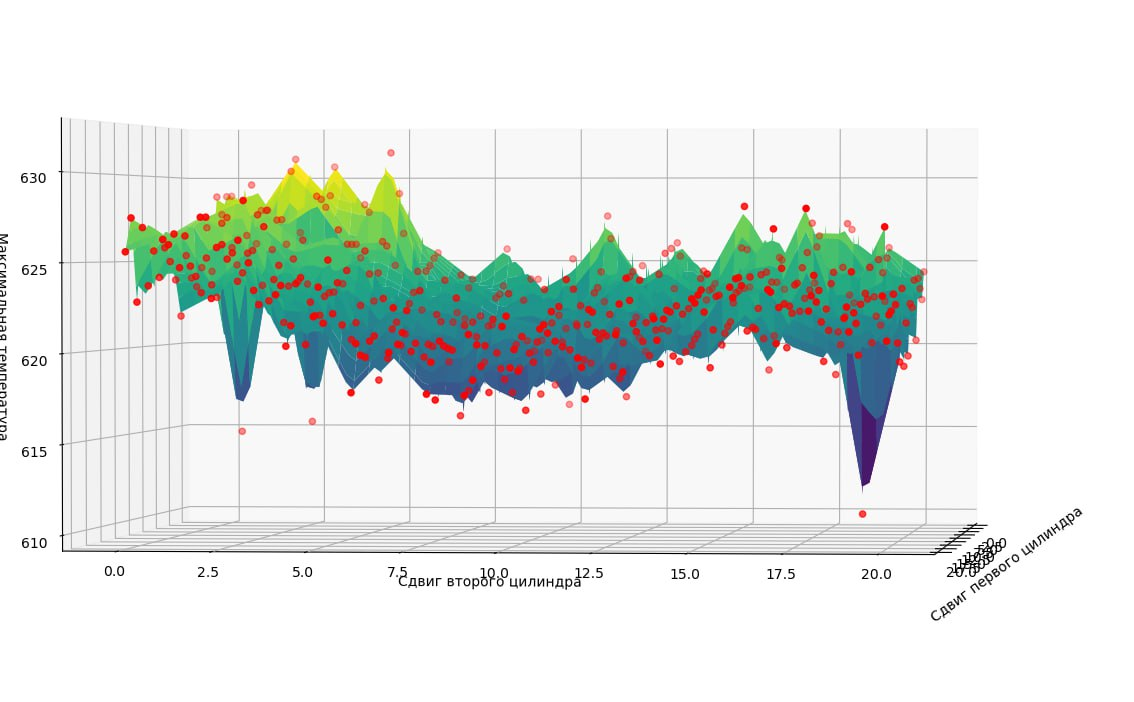
\includegraphics[width=0.4\linewidth]{images/22.2.jpg}
		\caption{Зависимость максимальной температуры нагревателя от сдвигов цилиндров} %% подпись к рисунку
	\end{center}
\end{figure}
\begin{figure}[h]
	\begin{center}
		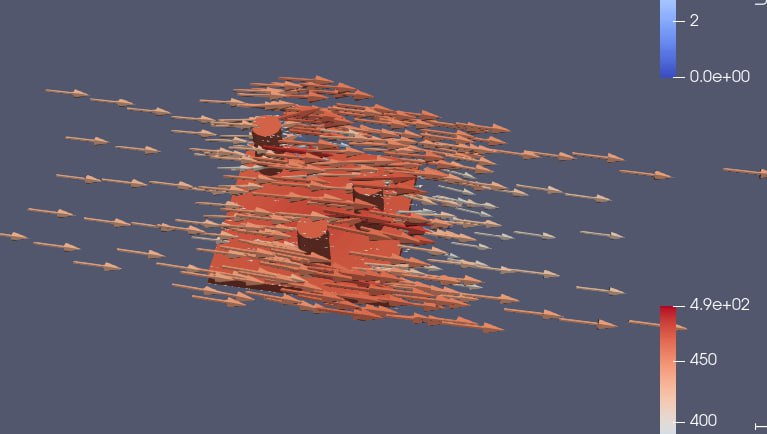
\includegraphics[width=0.4\linewidth]{images/22.3.jpg}
		\caption{Скорость течения} %% подпись к рисунку
	\end{center}
\end{figure}
\begin{figure}[h]
	\begin{center}
		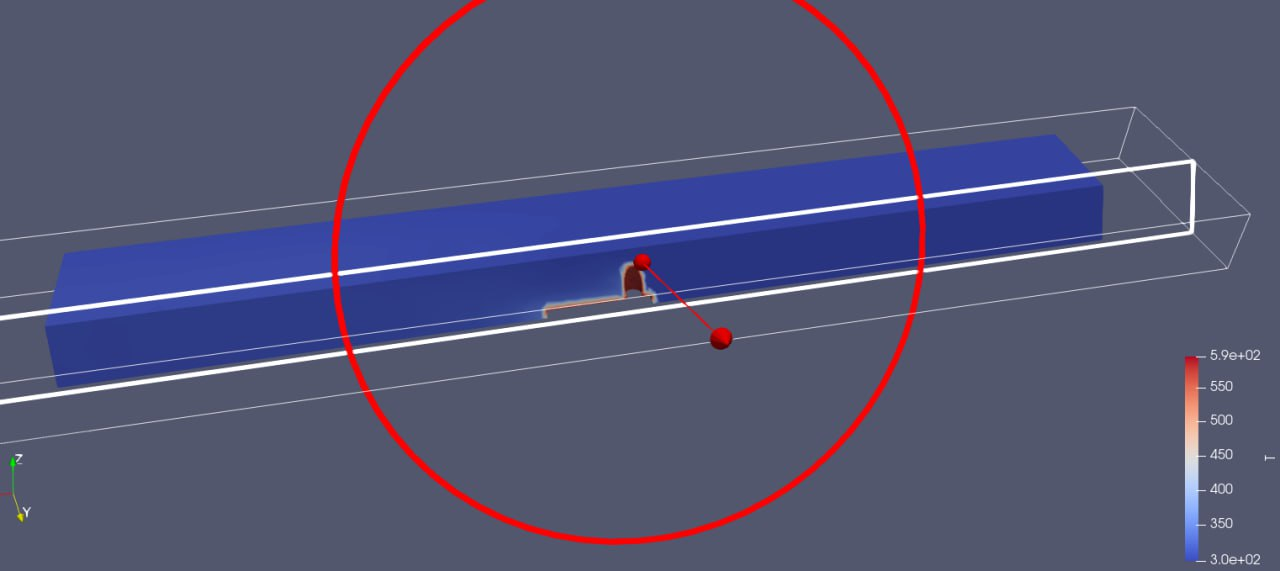
\includegraphics[width=0.4\linewidth]{images/22.4.jpg}
		\caption{Новая геометрия} %% подпись к рисунку
	\end{center}
\end{figure}

\section{Анализ реальной системы и изменения параметров}

Следующим этапом исследования стал анализ условий, представляющих реальную систему охлаждения. Внесенные изменения включали снижение скорости воздуха внутри воздуховода до 3 м/с (по сравнению с предыдущим значением 5.6 м/с), замену материала радиатора на медь (предыдущий материал - алюминий), а также модификацию геометрии нагревателя, сделав его тоньше и значительно больше по размерам, а саму подложку радиатора сделав толще.

\begin{figure}[h]
	\begin{center}
		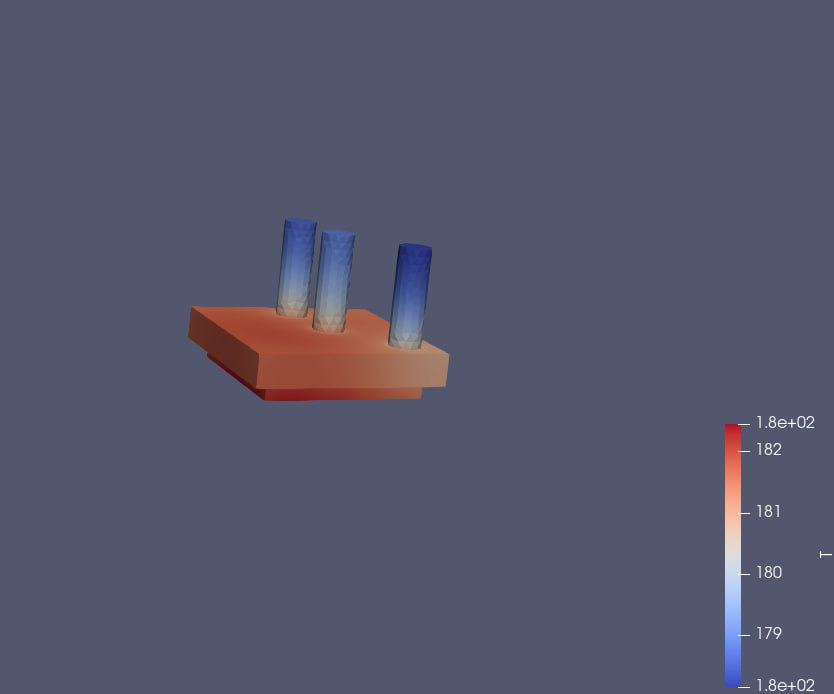
\includegraphics[width=0.4\linewidth]{images/23.1.jpg}
		\caption{Измененная геометрия} %% подпись к рисунку
	\end{center}
\end{figure}
\begin{figure}[h]
	\begin{center}
		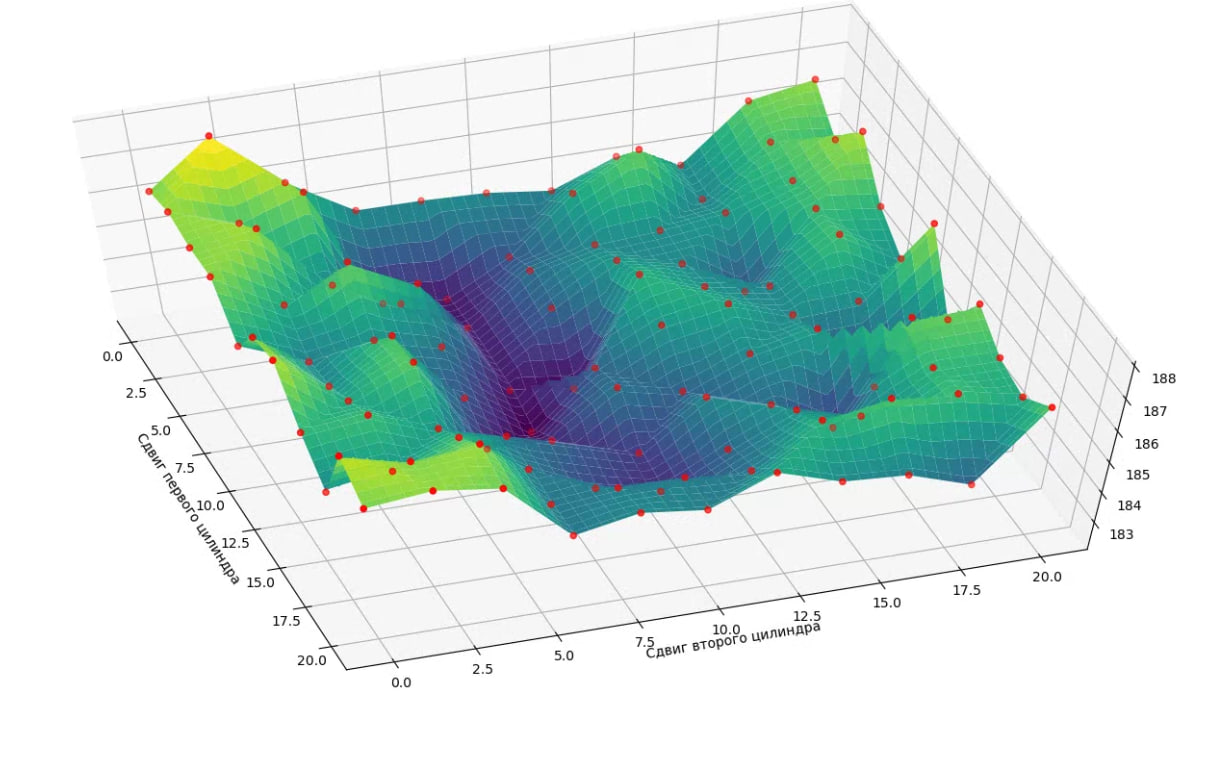
\includegraphics[width=0.4\linewidth]{images/23.2.jpg}
		\caption{Зависимость максимальной температуры нагревателя от сдвигов цилиндров} %% подпись к рисунку
	\end{center}
\end{figure}
\begin{figure}[h]
	\begin{center}
		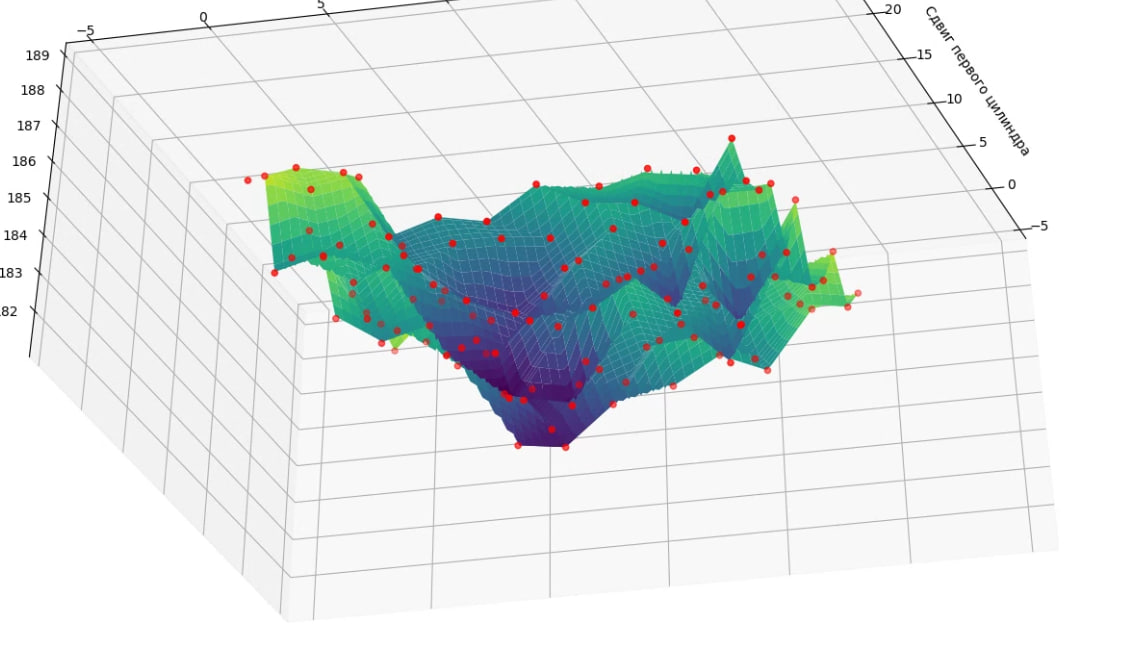
\includegraphics[width=0.4\linewidth]{images/23.3.jpg}
		\caption{Зависимость максимальной температуры нагревателя от сдвигов цилиндров} %% подпись к рисунку
	\end{center}
\end{figure}

\newpage
\section{Применение эволюционного алгоритма в оптимизации}

Необходимо отметить, что для более эффективного и быстрого поиска оптимальных параметров в задаче охлаждения был применен эволюционный алгоритм. Эволюционные алгоритмы — это класс методов оптимизации, вдохновленных процессами биологической эволюции. Они включают в себя механизмы отбора, скрещивания и мутации, а применительно к задачам оптимизации, такие алгоритмы позволяют находить оптимальные решения в пространствах больших размерностей.

Принцип работы эволюционного алгоритма можно кратко описать следующим образом:

\begin{enumerate}
	\item \textbf{Инициализация популяции:} Создается начальная популяция индивидов (наборов параметров) случайным образом или на основе каких-то эвристик.
	      
	\item \textbf{Оценка приспособленности:} Каждый индивид из популяции оценивается по степени приспособленности в соответствии с целевой функцией. В нашем контексте целевая функция - минимизация максимальной температуры внутри нагревателя.
	      
	\item \textbf{Отбор:} Выбираются наиболее приспособленные индивиды для следующего поколения. Это может происходить различными методами, такими как турнирный отбор, рулеточный отбор и др.
	      
	\item \textbf{Скрещивание:} Происходит кроссовер (скрещивание) между выбранными индивидами, что приводит к созданию новых индивидов. Это позволяет объединить положительные черты родителей.
	      
	\item \textbf{Мутация:} Некоторые индивиды могут подвергаться мутациям, изменяя свои параметры с определенной вероятностью. Это вносит элемент случайности и разнообразия в популяцию.
	      
	\item \textbf{Повторение:} Описанные шаги повторяются в цикле до достижения критерия остановки, такого как заданное количество поколений или достижение требуемой точности.
\end{enumerate}

Эволюционные алгоритмы являются мощным инструментом для оптимизации в больших пространствах параметров, позволяя находить приближенно оптимальные решения в условиях ограниченной информации о системе \cite{evolution}.

Применение эволюционного алгоритма в задаче оптимизации параметров системы охлаждения значительно снизило количество необходимых расчетов. Вместо полного перебора 121 точек в пространстве параметров, алгоритм смог достичь точек минимума всего за 50 расчетов.

\section{Использование градиентного метода}

Помимо дифференциальной эволюции, данная работа включала использование градиентного метода для оптимизации. Градиентные методы широко используются в численной оптимизации для поиска минимума (или максимума) функции. Они базируются на использовании градиента функции (вектора её частных производных) для определения направления поиска оптимального значения. Один из простых градиентных методов - это метод гради��нтного спуска.

\begin{enumerate}
	\item Инициализация параметров случайными значениями.
	\item Повторение до сходимости (или до достижения максимального числа итераций):
	      \begin{itemize}
		      \item Вычисление градиента функции по параметрам.
		      \item Обновление параметров в направлении, противоположном градиенту.
	      \end{itemize}
\end{enumerate}

Однако метод градиентного спуска может иметь ограничения, такие как сходимость к локальным минимумам или чувствительность к выбору начальных значений параметров \cite{Chernyshev2007}.

\begin{figure}[h]
	\begin{center}
		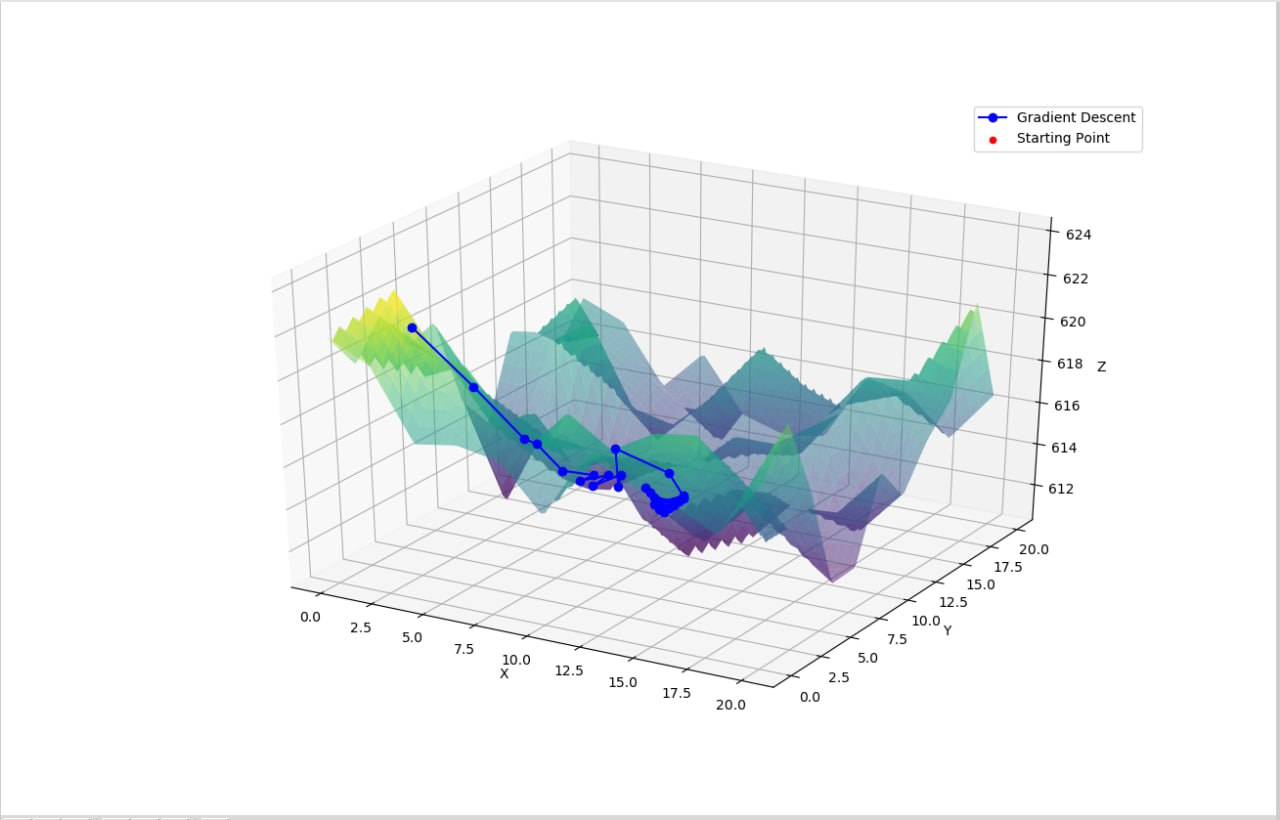
\includegraphics[width=0.4\linewidth]{images/24.jpg}
		\caption{Зависимость максимальной температуры нагревателя от сдвигов цилиндров} %% подпись к рисунку
	\end{center}
\end{figure}

L-BFGS-B (Limited-memory Broyden-Fletcher-Goldfarb-Shanno with Bound constraints):

L-BFGS-B - это усовершенствованный метод оптимизации, предназначенный для решения задач с ограничениями. Он поддерживает локальную оптимизацию с ограничениями на параметры.

\begin{enumerate}
	\item Ограничения:
	      \begin{itemize}
		      \item Метод позволяет оптимизировать функцию с учетом границ (ограничений) для параметров. Это важно, когда некоторые параметры должны оставаться в пределах определенных значений.
	      \end{itemize}
	\item Лимит памяти:
	      \begin{itemize}
		      \item "Limited-memory" в названии относится к тому, что метод хранит ограниченное количество предыдущих итераций для оценки гессиана. Это особенно полезно, когда размерность пространства параметров велика.
	      \end{itemize}
	\item BFGS-подобные обновления:
	      \begin{itemize}
		      \item Метод L-BFGS-B использует обновления BFGS для оценки обратного гессиана, что позволяет улучшить сходимость метода.
	      \end{itemize}
\end{enumerate}

Использование L-BFGS-B может быть предпочтительным, особенно при наличии ограничений на параметры. Этот метод часто применяется в задачах оптимизации, таких как подгонка параметров в статистических мо��елях или решение задач машинного обучения, где требуется минимизация функции потерь \cite{limited_BFGS}.

\newpage
\section*{Переход к доменному заполнению}
Следующим этапом стало доменное заполнение геометрии радиатора, для этого вся площадка радиатора была разделена на 36 частей.

\begin{figure}[h]
	\begin{center}
		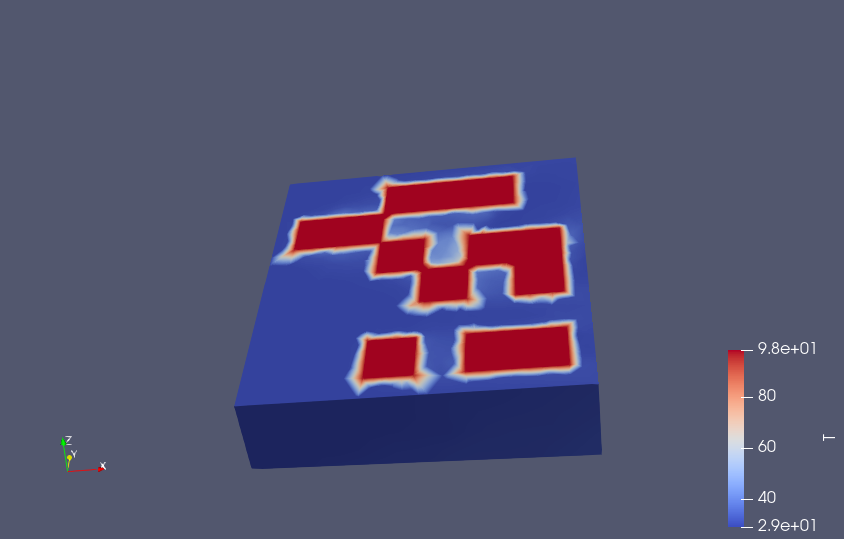
\includegraphics[width=0.4\linewidth]{images/25.1.png}
		\caption{Доменная геометрия распределение температуры} %% подпись к рисунку
	\end{center}
\end{figure}
\begin{figure}[h]
	\begin{center}
		\includegraphics[width=0.4\linewidth]{images/25.2.png}
		\caption{Доменная геометрия распределение скорости потока} %% подпись к рисунку
	\end{center}
\end{figure}

\newpage
\section*{Использование API ParaView для создания анимации}

На данном этапе использовалось API ParaView, с его помощью автоматизировался процессы анализа и визуализации полученных данных.
Код представлен в приложении.

\newpage
\section*{Изменение входного и выходного отверстия}


\newpage
\section*{Заключение}

В ходе данной работы было проведено комплексное исследование системы охлаждения с использованием численных методов и оптимизации. Основные выводы и результаты работы:

\begin{enumerate}
	\item \textbf{Геометрические изменения:} проведен анализ геометрии системы, выполнено исследование влияния расположения цилиндров на эффективность охлаждения. Эксперименты с различными конфигурациями позволили выявить оптимальные расстановки и влияние контакта цилиндров друг с другом на тепловые характеристики.
	      
	\item \textbf{Оптимизация с использованием полного перебора:} проведена первоначальная оптимизация системы, использован полный перебор, что позволило выявить оптимальные точки в пространстве параметров. Это дало общий обзор зависимостей и минимумов целевой функции.
	      
	\item \textbf{Многопоточность для улучшения производительности:} в процессе увеличения количества точек в пространстве параметров использовалась многопоточность для оптимизации, что значительно ускорило процесс расчета и позволило нам провести более подробное исследование.
	      
	\item \textbf{Изменения в геометрии и параметрах системы:}исследовали влияние различных параметров, таких как скорость воздуха и материалы, на эффективность охлаждения. Изменения в геометрии и па��аметрах системы привели к новым интересным результатам, позволяя лучше понять зависимости и оптимизировать систему.
	      
	\item \textbf{Эволюционный алгоритм:} применили эвол��ционный алгоритм для оптимизации системы. Этот метод позволил более эффективно находить точки минимума, снижая количество расчетов по сравнению с полным перебором.
	      
	\item \textbf{Градиентные методы оптимизации:} использование градиентных методов, таких как L-BFGS-B, добавило эффективность и точность в арсенал оптимизационных методов.
	      
	\item \textbf{Выводы и перспективы:} на основе результатов исследования необходимо сделать вывод о том, что оптимизация геометрии и параметров системы охлаждения может существенно повысить ее эффективность. Подход с использованием различных методов оптимизации и численного моделирования предоставляет мощный инструментарий для разработки и улучшения теплоотводящих систем. В будущем возможно проведение более глубоких исследований с учетом дополнительных факторов и условий эксплуатации системы.
\end{enumerate}

\newpage
\bibliographystyle{utf8gost705u}  %% стилевой файл для оформления по ГОСТу
\bibliography{Overview}     %% имя библиографической базы (bib-файл) 

\newpage
\section*{Приложение А}
% \renewcommand{\thesection}{\Asbuk{section}}
Проект можно найти на github (github.com/AlexEsn/FOAM\_project), где с��держатся все скрипты и кейсы.

\end{document}